
%% bare_conf.tex
%% V1.4b
%% 2015/08/26
%% by Michael Shell
%% See:
%% http://www.michaelshell.org/
%% for current contact information.
%%
%% This is a skeleton file demonstrating the use of IEEEtran.cls
%% (requires IEEEtran.cls version 1.8b or later) with an IEEE
%% conference paper.
%%
%% Support sites:
%% http://www.michaelshell.org/tex/ieeetran/
%% http://www.ctan.org/pkg/ieeetran
%% and
%% http://www.ieee.org/

%%*************************************************************************
%% Legal Notice:
%% This code is offered as-is without any warranty either expressed or
%% implied; without even the implied warranty of MERCHANTABILITY or
%% FITNESS FOR A PARTICULAR PURPOSE! 
%% User assumes all risk.
%% In no event shall the IEEE or any contributor to this code be liable for
%% any damages or losses, including, but not limited to, incidental,
%% consequential, or any other damages, resulting from the use or misuse
%% of any information contained here.
%%
%% All comments are the opinions of their respective authors and are not
%% necessarily endorsed by the IEEE.
%%
%% This work is distributed under the LaTeX Project Public License (LPPL)
%% ( http://www.latex-project.org/ ) version 1.3, and may be freely used,
%% distributed and modified. A copy of the LPPL, version 1.3, is included
%% in the base LaTeX documentation of all distributions of LaTeX released
%% 2003/12/01 or later.
%% Retain all contribution notices and credits.
%% ** Modified files should be clearly indicated as such, including  **
%% ** renaming them and changing author support contact information. **
%%*************************************************************************


% *** Authors should verify (and, if needed, correct) their LaTeX system  ***
% *** with the testflow diagnostic prior to trusting their LaTeX platform ***
% *** with production work. The IEEE's font choices and paper sizes can   ***
% *** trigger bugs that do not appear when using other class files.       ***                          ***
% The testflow support page is at:
% http://www.michaelshell.org/tex/testflow/


\documentclass[conference]{IEEEtran}
% Some Computer Society conferences also require the compsoc mode option,
% but others use the standard conference format.
%
% If IEEEtran.cls has not been installed into the LaTeX system files,
% manually specify the path to it like:
% \documentclass[conference]{../sty/IEEEtran}


% Some very useful LaTeX packages include:
% (uncomment the ones you want to load)

\usepackage{makecell}
%Så vi kan få flere linjer i tabeller
\usepackage{multirow}
%Så vi kan lave flere rækker i cellerne 

\usepackage[hidelinks]{hyperref}
%Så der ikke er en kasse rundt om links til henvisninger mm. 

\usepackage{color}
%Så vi kan skrive tekst i forskellige farver. 

\usepackage{ulem}
%Så man kan lave en streg gennem teksten. 

\usepackage[utf8]{inputenc}
%Så vi kan skrive æ,ø og å 

\usepackage[footnote,marginclue,draft,danish,silent,nomargin]{fixme}
%Muliggør kommentarer. Udskift evt. "draft" med "final" for at udløse en fejl ved typesætning




% *** MISC UTILITY PACKAGES ***
%
\usepackage{ifpdf}
% Heiko Oberdiek's ifpdf.sty is very useful if you need conditional
% compilation based on whether the output is pdf or dvi.
% usage:
% \ifpdf
%   % pdf code
% \else
%   % dvi code
% \fi
% The latest version of ifpdf.sty can be obtained from:
% http://www.ctan.org/pkg/ifpdf
% Also, note that IEEEtran.cls V1.7 and later provides a builtin
% \ifCLASSINFOpdf conditional that works the same way.
% When switching from latex to pdflatex and vice-versa, the compiler may
% have to be run twice to clear warning/error messages.



% *** CITATION PACKAGES ***
%
\usepackage{cite}
% cite.sty was written by Donald Arseneau
% V1.6 and later of IEEEtran pre-defines the format of the cite.sty package
% \cite{} output to follow that of the IEEE. Loading the cite package will
% result in citation numbers being automatically sorted and properly
% "compressed/ranged". e.g., [1], [9], [2], [7], [5], [6] without using
% cite.sty will become [1], [2], [5]--[7], [9] using cite.sty. cite.sty's
% \cite will automatically add leading space, if needed. Use cite.sty's
% noadjust option (cite.sty V3.8 and later) if you want to turn this off
% such as if a citation ever needs to be enclosed in parenthesis.
% cite.sty is already installed on most LaTeX systems. Be sure and use
% version 5.0 (2009-03-20) and later if using hyperref.sty.
% The latest version can be obtained at:
% http://www.ctan.org/pkg/cite
% The documentation is contained in the cite.sty file itself.


\usepackage{hyperref}
%Så vi kan referer til figur, tabel mm. med f.eks. Figure 1 - autoref

% *** GRAPHICS RELATED PACKAGES ***
%
%\ifCLASSINFOpdf
 \usepackage[pdftex]{graphicx}
%  % declare the path(s) where your graphic files are
%  % \graphicspath{{../pdf/}{../jpeg/}}
%  % and their extensions so you won't have to specify these with
%  % every instance of \includegraphics
%  % \DeclareGraphicsExtensions{.pdf,.jpeg,.png}
%\else
%  % or other class option (dvipsone, dvipdf, if not using dvips). graphicx
%  % will default to the driver specified in the system graphics.cfg if no
%  % driver is specified.
%  % \usepackage[dvips]{graphicx}
%  % declare the path(s) where your graphic files are
%  % \graphicspath{{../eps/}}
%  % and their extensions so you won't have to specify these with
%  % every instance of \includegraphics
%  % \DeclareGraphicsExtensions{.eps}
%\fi
% graphicx was written by David Carlisle and Sebastian Rahtz. It is
% required if you want graphics, photos, etc. graphicx.sty is already
% installed on most LaTeX systems. The latest version and documentation
% can be obtained at: 
% http://www.ctan.org/pkg/graphicx
% Another good source of documentation is "Using Imported Graphics in
% LaTeX2e" by Keith Reckdahl which can be found at:
% http://www.ctan.org/pkg/epslatex
%
% latex, and pdflatex in dvi mode, support graphics in encapsulated
% postscript (.eps) format. pdflatex in pdf mode supports graphics
% in .pdf, .jpeg, .png and .mps (metapost) formats. Users should ensure
% that all non-photo figures use a vector format (.eps, .pdf, .mps) and
% not a bitmapped formats (.jpeg, .png). The IEEE frowns on bitmapped formats
% which can result in "jaggedy"/blurry rendering of lines and letters as
% well as large increases in file sizes.
%
% You can find documentation about the pdfTeX application at:
% http://www.tug.org/applications/pdftex



% *** MATH PACKAGES ***
%
\usepackage{amsmath}
% A popular package from the American Mathematical Society that provides
% many useful and powerful commands for dealing with mathematics.
%
% Note that the amsmath package sets \interdisplaylinepenalty to 10000
% thus preventing page breaks from occurring within multiline equations. Use:
%\interdisplaylinepenalty=2500
% after loading amsmath to restore such page breaks as IEEEtran.cls normally
% does. amsmath.sty is already installed on most LaTeX systems. The latest
% version and documentation can be obtained at:
% http://www.ctan.org/pkg/amsmath



% *** SPECIALIZED LIST PACKAGES ***
%
%\usepackage{algorithmic}
% algorithmic.sty was written by Peter Williams and Rogerio Brito.
% This package provides an algorithmic environment fo describing algorithms.
% You can use the algorithmic environment in-text or within a figure
% environment to provide for a floating algorithm. Do NOT use the algorithm
% floating environment provided by algorithm.sty (by the same authors) or
% algorithm2e.sty (by Christophe Fiorio) as the IEEE does not use dedicated
% algorithm float types and packages that provide these will not provide
% correct IEEE style captions. The latest version and documentation of
% algorithmic.sty can be obtained at:
% http://www.ctan.org/pkg/algorithms
% Also of interest may be the (relatively newer and more customizable)
% algorithmicx.sty package by Szasz Janos:
% http://www.ctan.org/pkg/algorithmicx



% *** ALIGNMENT PACKAGES ***
%
\usepackage{array}
% Frank Mittelbach's and David Carlisle's array.sty patches and improves
% the standard LaTeX2e array and tabular environments to provide better
% appearance and additional user controls. As the default LaTeX2e table
% generation code is lacking to the point of almost being broken with
% respect to the quality of the end results, all users are strongly
% advised to use an enhanced (at the very least that provided by array.sty)
% set of table tools. array.sty is already installed on most systems. The
% latest version and documentation can be obtained at:
% http://www.ctan.org/pkg/array


% IEEEtran contains the IEEEeqnarray family of commands that can be used to
% generate multiline equations as well as matrices, tables, etc., of high
% quality.




% *** SUBFIGURE PACKAGES ***
%\ifCLASSOPTIONcompsoc
%  \usepackage[caption=false,font=normalsize,labelfont=sf,textfont=sf]{subfig}
%\else
%  \usepackage[caption=false,font=footnotesize]{subfig}
%\fi
% subfig.sty, written by Steven Douglas Cochran, is the modern replacement
% for subfigure.sty, the latter of which is no longer maintained and is
% incompatible with some LaTeX packages including fixltx2e. However,
% subfig.sty requires and automatically loads Axel Sommerfeldt's caption.sty
% which will override IEEEtran.cls' handling of captions and this will result
% in non-IEEE style figure/table captions. To prevent this problem, be sure
% and invoke subfig.sty's "caption=false" package option (available since
% subfig.sty version 1.3, 2005/06/28) as this is will preserve IEEEtran.cls
% handling of captions.
% Note that the Computer Society format requires a larger sans serif font
% than the serif footnote size font used in traditional IEEE formatting
% and thus the need to invoke different subfig.sty package options depending
% on whether compsoc mode has been enabled.
%
% The latest version and documentation of subfig.sty can be obtained at:
% http://www.ctan.org/pkg/subfig




% *** FLOAT PACKAGES ***
%
\usepackage{float}

% \usepackage{fixltx2e}
% fixltx2e, the successor to the earlier fix2col.sty, was written by
% Frank Mittelbach and David Carlisle. This package corrects a few problems
% in the LaTeX2e kernel, the most notable of which is that in current
% LaTeX2e releases, the ordering of single and double column floats is not
% guaranteed to be preserved. Thus, an unpatched LaTeX2e can allow a
% single column figure to be placed prior to an earlier double column
% figure.
% Be aware that LaTeX2e kernels dated 2015 and later have fixltx2e.sty's
% corrections already built into the system in which case a warning will
% be issued if an attempt is made to load fixltx2e.sty as it is no longer
% needed.
% The latest version and documentation can be found at:
% http://www.ctan.org/pkg/fixltx2e


\usepackage{stfloats}
% stfloats.sty was written by Sigitas Tolusis. This package gives LaTeX2e
% the ability to do double column floats at the bottom of the page as well
% as the top. (e.g., "\begin{figure*}[!b]" is not normally possible in
% LaTeX2e). It also provides a command:
%\fnbelowfloat
% to enable the placement of footnotes below bottom floats (the standard
% LaTeX2e kernel puts them above bottom floats). This is an invasive package
% which rewrites many portions of the LaTeX2e float routines. It may not work
% with other packages that modify the LaTeX2e float routines. The latest
% version and documentation can be obtained at:
% http://www.ctan.org/pkg/stfloats
% Do not use the stfloats baselinefloat ability as the IEEE does not allow
% \baselineskip to stretch. Authors submitting work to the IEEE should note
% that the IEEE rarely uses double column equations and that authors should try
% to avoid such use. Do not be tempted to use the cuted.sty or midfloat.sty
% packages (also by Sigitas Tolusis) as the IEEE does not format its papers in
% such ways.
% Do not attempt to use stfloats with fixltx2e as they are incompatible.
% Instead, use Morten Hogholm'a dblfloatfix which combines the features
% of both fixltx2e and stfloats:
%
% \usepackage{dblfloatfix}
% The latest version can be found at:
% http://www.ctan.org/pkg/dblfloatfix




% *** PDF, URL AND HYPERLINK PACKAGES ***
%
\usepackage{url}
% url.sty was written by Donald Arseneau. It provides better support for
% handling and breaking URLs. url.sty is already installed on most LaTeX
% systems. The latest version and documentation can be obtained at:
% http://www.ctan.org/pkg/url
% Basically, \url{my_url_here}.




% *** Do not adjust lengths that control margins, column widths, etc. ***
% *** Do not use packages that alter fonts (such as pslatex).         ***
% There should be no need to do such things with IEEEtran.cls V1.6 and later.
% (Unless specifically asked to do so by the journal or conference you plan
% to submit to, of course. )


% correct bad hyphenation here
\hyphenation{op-tical net-works semi-conduc-tor}


\begin{document}
%
% paper title
% Titles are generally capitalized except for words such as a, an, and, as,
% at, but, by, for, in, nor, of, on, or, the, to and up, which are usually
% not capitalized unless they are the first or last word of the title.
% Linebreaks \\ can be used within to get better formatting as desired.
% Do not put math or special symbols in the title.
\title{Subjective Experience of Interacting \\ with a Social Robot at a Danish Airport}


% author names and affiliations
% use a multiple column layout for up to three different
% affiliations
%\author{\IEEEauthorblockN{Michael Shell}
%\IEEEauthorblockA{School of Electrical and\\Computer Engineering\\
%Georgia Institute of Technology\\
%Atlanta, Georgia 30332--0250\\
%Email: http://www.michaelshell.org/contact.html}
%\and
%\IEEEauthorblockN{Homer Simpson}
%\IEEEauthorblockA{Twentieth Century Fox\\
%Springfield, USA\\
%Email: homer@thesimpsons.com}
%\and
%\IEEEauthorblockN{James Kirk\\ and Montgomery Scott}
%\IEEEauthorblockA{Starfleet Academy\\
%San Francisco, California 96678--2391\\
%Telephone: (800) 555--1212\\
%Fax: (888) 555--1212}}

% conference papers do not typically use \thanks and this command
% is locked out in conference mode. If really needed, such as for
% the acknowledgment of grants, issue a \IEEEoverridecommandlockouts
% after \documentclass

% for over three affiliations, or if they all won't fit within the width
% of the page, use this alternative format:
% 
\author{\IEEEauthorblockN{Andreas Kornmaaler Hansen\IEEEauthorrefmark{0},
Emil Bonnerup\IEEEauthorrefmark{0},
Juliane Nilsson\IEEEauthorrefmark{0}, 
Lucca Julie Nellemann,\IEEEauthorrefmark{0} and
Sara Nielsen\IEEEauthorrefmark{0}}
\IEEEauthorblockA{\IEEEauthorrefmark{0}School of Information and Communication Technology\\
Aalborg University,
Aalborg, Denmark\\ Email: 17gr782@es.aau.dk}
}


\makeatletter
\def\bstctlcite{\@ifnextchar[{\@bstctlcite}{\@bstctlcite[@auxout]}}
\def\@bstctlcite[#1]#2{\@bsphack
  \@for\@citeb:=#2\do{%
    \edef\@citeb{\expandafter\@firstofone\@citeb}%
    \if@filesw\immediate\write\csname #1\endcsname{\string\citation{\@citeb}}\fi}%
  \@esphack}
\makeatother

% use for special paper notices
\IEEEspecialpapernotice{Unpublished Conference Paper for SEMCON at Aalborg University 2017}

% make the title area
\maketitle
\thispagestyle{plain}
\pagestyle{plain}
% As a general rule, do not put math, special symbols or citations
% in the abstract
\begin{abstract}
\label{Abstract}
% As a general rule, do not put math, special symbols or citations
% in the abstract
Social robots are expected to play a much bigger role in the near future. This calls for research in determining how these social robots are supposed to behave. This paper presents an ecological field study and investigates the subjective experience of social robots in Aalborg Airport (AAL). Travellers were recruited by a remote controlled robot from Double Robotics, Inc., which had a tablet with an interface asking if it may help them with wayfinding in AAL. When the participants had chosen their location they were asked to follow the robot and led to a semi-structured interview about their first impressions. In total the study includes 30 participants from 8 to 62 years (M=37.9, SD=17.1). The observations and the participants' statements were coded using an Affinity Diagram. 567 affinity notes were sorted and ended up with 10 categories of which the main categories revolved around appearance, behaviour, approach and trust. 


%method
%result
%conclusion

\end{abstract}

% no keywords

% For peer review papers, you can put extra information on the cover
% page as needed:
% \ifCLASSOPTIONpeerreview
% \begin{center} \bfseries EDICS Category: 3-BBND \end{center}
% \fi
%
% For peerreview papers, this IEEEtran command inserts a page break and
% creates the second title. It will be ignored for other modes.
\IEEEpeerreviewmaketitle

\chapter*{Introduction}
\label{introduction}
%
The goal of this paper is to analyse results from a study called \textit{Men and Bread} using Principal Component Analysis (PCA). \blankline
% 
<<<<<<< HEAD
In the study \textit{Men and Bread}, 21 subjects were asked to rate different types of buns according to different attributes. Nine different types of buns were presented, where one was presented as a familiarization with the scales. The buns presented in the study are shown in \autoref{fig:bread}, where bread B9 is the bun used for familiarization. 
=======
In the study \textit{Men and Bread} 21 subjects were asked to rate nine different types of buns according to different attributes. Nine different types of buns were presented where one was presented as a familiarization with the scales. The buns presented in the study are shown on \autoref{fig:bread}, where bread B9 is the bun used for familiarization. 
>>>>>>> ad024fa761c2fdb0b59931c6f6a1eb4b88ee637a
%
\begin{figure}[H]
\centering
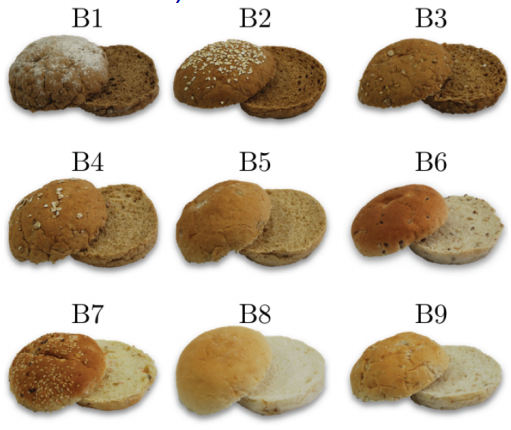
\includegraphics[width =0.7\textwidth]{Figure/Bread}
\caption{The different types of buns with identifying name, presented so that both crust and crumb can be seen.}
\label{fig:bread}
\end{figure}
\noindent
%
For each one of the different types of buns, 11 different attributes grouped in three different categories were rated. The attributes with the belonging scale question for each category are presented in \autoref{tab:DirectPerception}, \autoref{tab:AbstractPerception}, and \autoref{tab:Reflection}.
%
\begin{table}[H]
	\centering 
	\begin{tabular}{ |l|l| }
	\hline
	\multicolumn{2}{ |c| }{\textbf{Direct perception}} \\
	\hline
	\textit{Attribute} & \textit{Scale Question} \\ 
	\hline
	\multirow{2}{*}{Crust} & Hvilken farve har skorpen? (lys til mørk) \\
 	&  What color is the crust? (light to dark) \\ \hline
	\multirow{2}{*}{Crumb} &  Hvilken farve har krummen? (lys til mørk) \\
 	&  What color is the crumb? (light to dark) \\ \hline
	\multirow{2}{*}{Surface} & Hvilken tekstur har overfladen? (glat til ujævn) \\
 	&  What texture does the surface have? (smooth to uneven) \\ \hline
	\multirow{2}{*}{Seeds} & Hvor stor er andelen af kerner? (lav til høj) \\ 
 	&  How great is the amount of seeds? (small to large)\\ 
	\hline
	\end{tabular}
	\caption{Scale questions under the category: Direct perception. This category of questions are related to the readily available aspects of the bread.}
	\label{tab:DirectPerception}       
\end{table}
\noindent
%
\begin{table}[H]
	\centering 
	\begin{tabular}{ |l|l| }
	\hline
	\multicolumn{2}{ |c| }{\textbf{Abstract perception}} \\
	\hline
	\textit{Attribute} & \textit{Scale Question} \\ 
	\hline
	\multirow{2}{*}{Weight} &  Hvor tungt er brødet? (let til tungt) \\
 	&  How weighty is the bread? (light to heavy) \\ \hline
	\multirow{2}{*}{Density} & Hvor tæt er brødet? (luftigt til kompakt) \\
 	&  How dense is the bread? (airy to dense) \\ \hline
	\multirow{2}{*}{Juicy} &  Hvor saftigt er brødet? (tørt til svampet) \\
 	&  How juicy is the bread? (dry to moist) \\ 
 	\hline
	\end{tabular}
	\caption{Scale questions under the category: Abstract perception. This category relates to slightly more abstract concepts where the visual sense might not be the best tool for investigation.}
	\label{tab:AbstractPerception}       
\end{table}
\noindent
%
\begin{table}[H]
	\centering 
	\begin{tabular}{ |l|l| }
	\hline
	\multicolumn{2}{ |c| }{\textbf{Reflection}} \\
	\hline
	\textit{Attribute} & \textit{Scale Question} \\ 
	\hline
	\multirow{2}{*}{Filling} & Hvor mættende ser brødet ud? (lidt til meget) \\
 	&  How filling is the bread? (a little to a lot) \\ \hline
	\multirow{2}{*}{Nourishing} & Hvor nærende ser brødet ud? (usundt til sundt) \\
 	&   How nourishing is the bread? (healthy to unhealthy) \\ \hline
	\multirow{2}{*}{Wholegrain} & Hvor fuldkornsholdigt er brødet? (lidt til meget) \\
 	&   How large is the amount of wholegrain in the bread? (low to high) \\ \hline
	\multirow{2}{*}{Fibre} & Hvor fiberholdigt er brødet? (lidt til meget) \\ 
 	&   How fibrous is the bread? (low to high))\\ 
	\hline
	\end{tabular}
	\caption{Scale questions under the category: Reflection. This category concerns the qualities associated with bread. Qualities which are assumed to require a level of reflection.}
	\label{tab:Reflection}       
\end{table}
\noindent
%
Each scale question were presented to the test subjects with a scale. The scale used to rate the buns was a \textit{Visual Analogue Scale} (VAS) with open endpoints and an anchor point in the middle. An example of the scale used in the study is shown on \autoref{fig:Skala}. 
%
\begin{figure}[H]
\centering
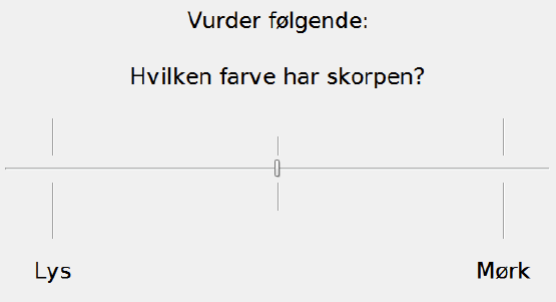
\includegraphics[width =0.7\textwidth]{Figure/Skala}
\caption{Example of the VAS used in the study \textit{Men and Bread}.}
\label{fig:Skala}
\end{figure}
\noindent


%Analyze the results from the example using PCA.

%First plot a “profile” of all stimuli.

%How much of the variance is explained by each component?

%(Plot a scree-plot including cumulative variance).

%Plot your PCA solution graphically. Both a plot with just your stimuli (scores) and a biplot with both scores and loadings.

%Make a table of the loadings of each word-pair on each principal component.

%Interpret the solution. Also, are there word-pairs that seem ”redundant” e.g. measures that same perceptual attribute?

\section{Method - Elicitation of attributes}
\label{MethodElicitation}
%
The first test was conducted on Danish travellers who interacted with a social robot in a natural setting. The test was conducted at Aalborg Airport (AAL) after the security check and before they reached the shopping and dining area at the airport. The travellers who interacted with the robot were asked to participate in a semi-structured interview about their first impressions while being observed during both the interaction and the interview. 

\subsection{Materials}
For the test a \textit{Double} robot from Double Robotics Inc, \cite{WEB:Double}, with an iPad Air 2, \cite{WEB:iPadAir2}, was used. Based on an small pretest it was decided to change the head mount so that the iPad is angled upwards, to make the robot appear more welcoming. The modified \textit{Double} robot is shown on \autoref{fig:ModificeretDoubleFront} and \autoref{fig:ModificeretDoubleSideClose}. The \textit{Double} robot was connected to a laptop via Wi-Fi connection and its own software. The \textit{Double} application allows a web page to be superimposed on the iPad screen while the controller is still able to control the robot from the laptop. The web page presented on the iPad was a wireframe developed in Marvel, (\url{www.marvelapp.com}), aiming to depict the potential usage of the robot as a wayfinding tool at AAL. The entire wireframe was formulated in Danish.

\subsection{Subject Recruitment}
30 subjects from the age of 8 to 62 years (M=37.9, SD=17.1) distributed among 16 females and 14 males participated. The subjects were recruited by the robot itself, which was remote controlled by a present controller, to provide a more ecological and undisturbed interaction between robot and subject. The robot approached potential subjects and the wireframe on the iPad asked them if it might help them find their way around AAL and presented a "Yes/No" option. If "No" was pressed, the robot wished the traveller a pleasent journey and left. If "Yes" was pressed, the subjects were presented with four wayfinding options: Food, Shopping, Toilets, or Gate information, as shown on \autoref{fig:brug}. The subjects were then kindly asked to follow the robot after they had chosen their preferred option. The robot then led the subjects to an interviewer who shortly informed them of the study and received verbal consent to record audio during the semi-structured interview. In total 18 interviews were conducted of which 11 were on single travellers and seven were on groups of travellers.
%
\begin{figure}[H]
\centering
\begin{minipage}{.25\textwidth}
  \centering
  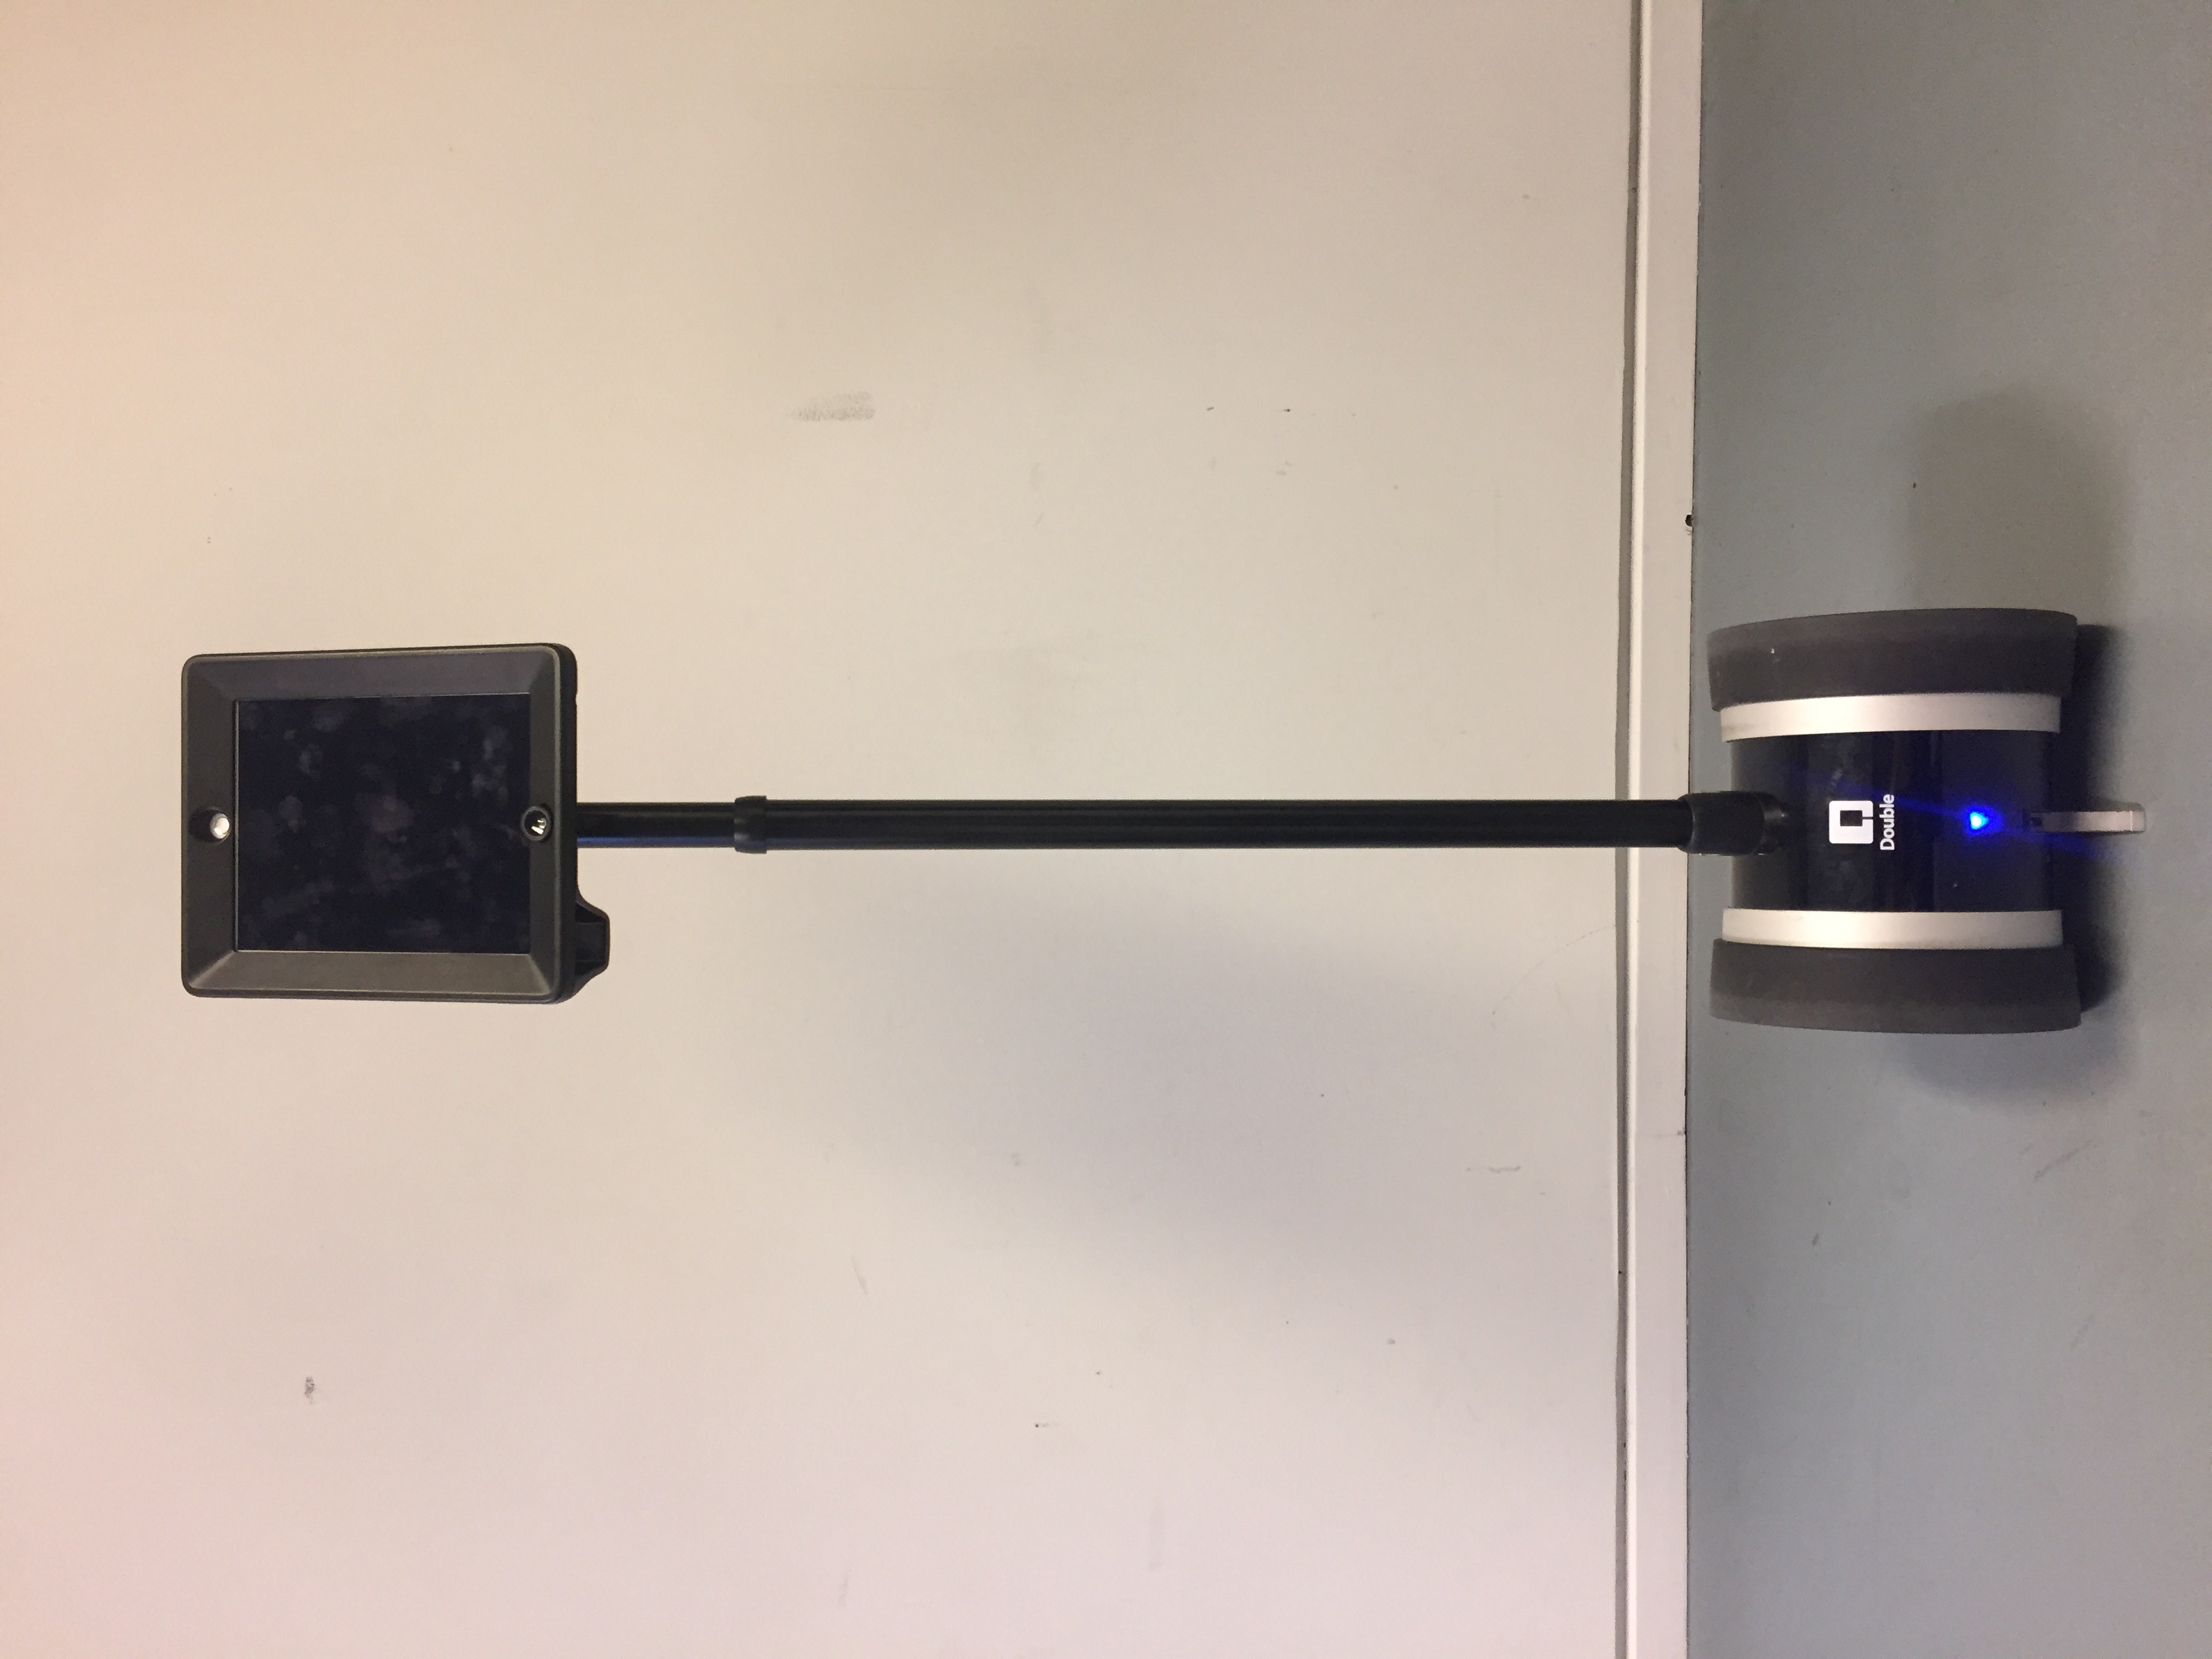
\includegraphics[width=\linewidth, angle =-90]{Figure/ModificeretDoubleFront}
  \caption{\textit{Double}'s front.}
  \label{fig:ModificeretDoubleFront}
\end{minipage}%
\begin{minipage}{.25\textwidth}
  \centering
  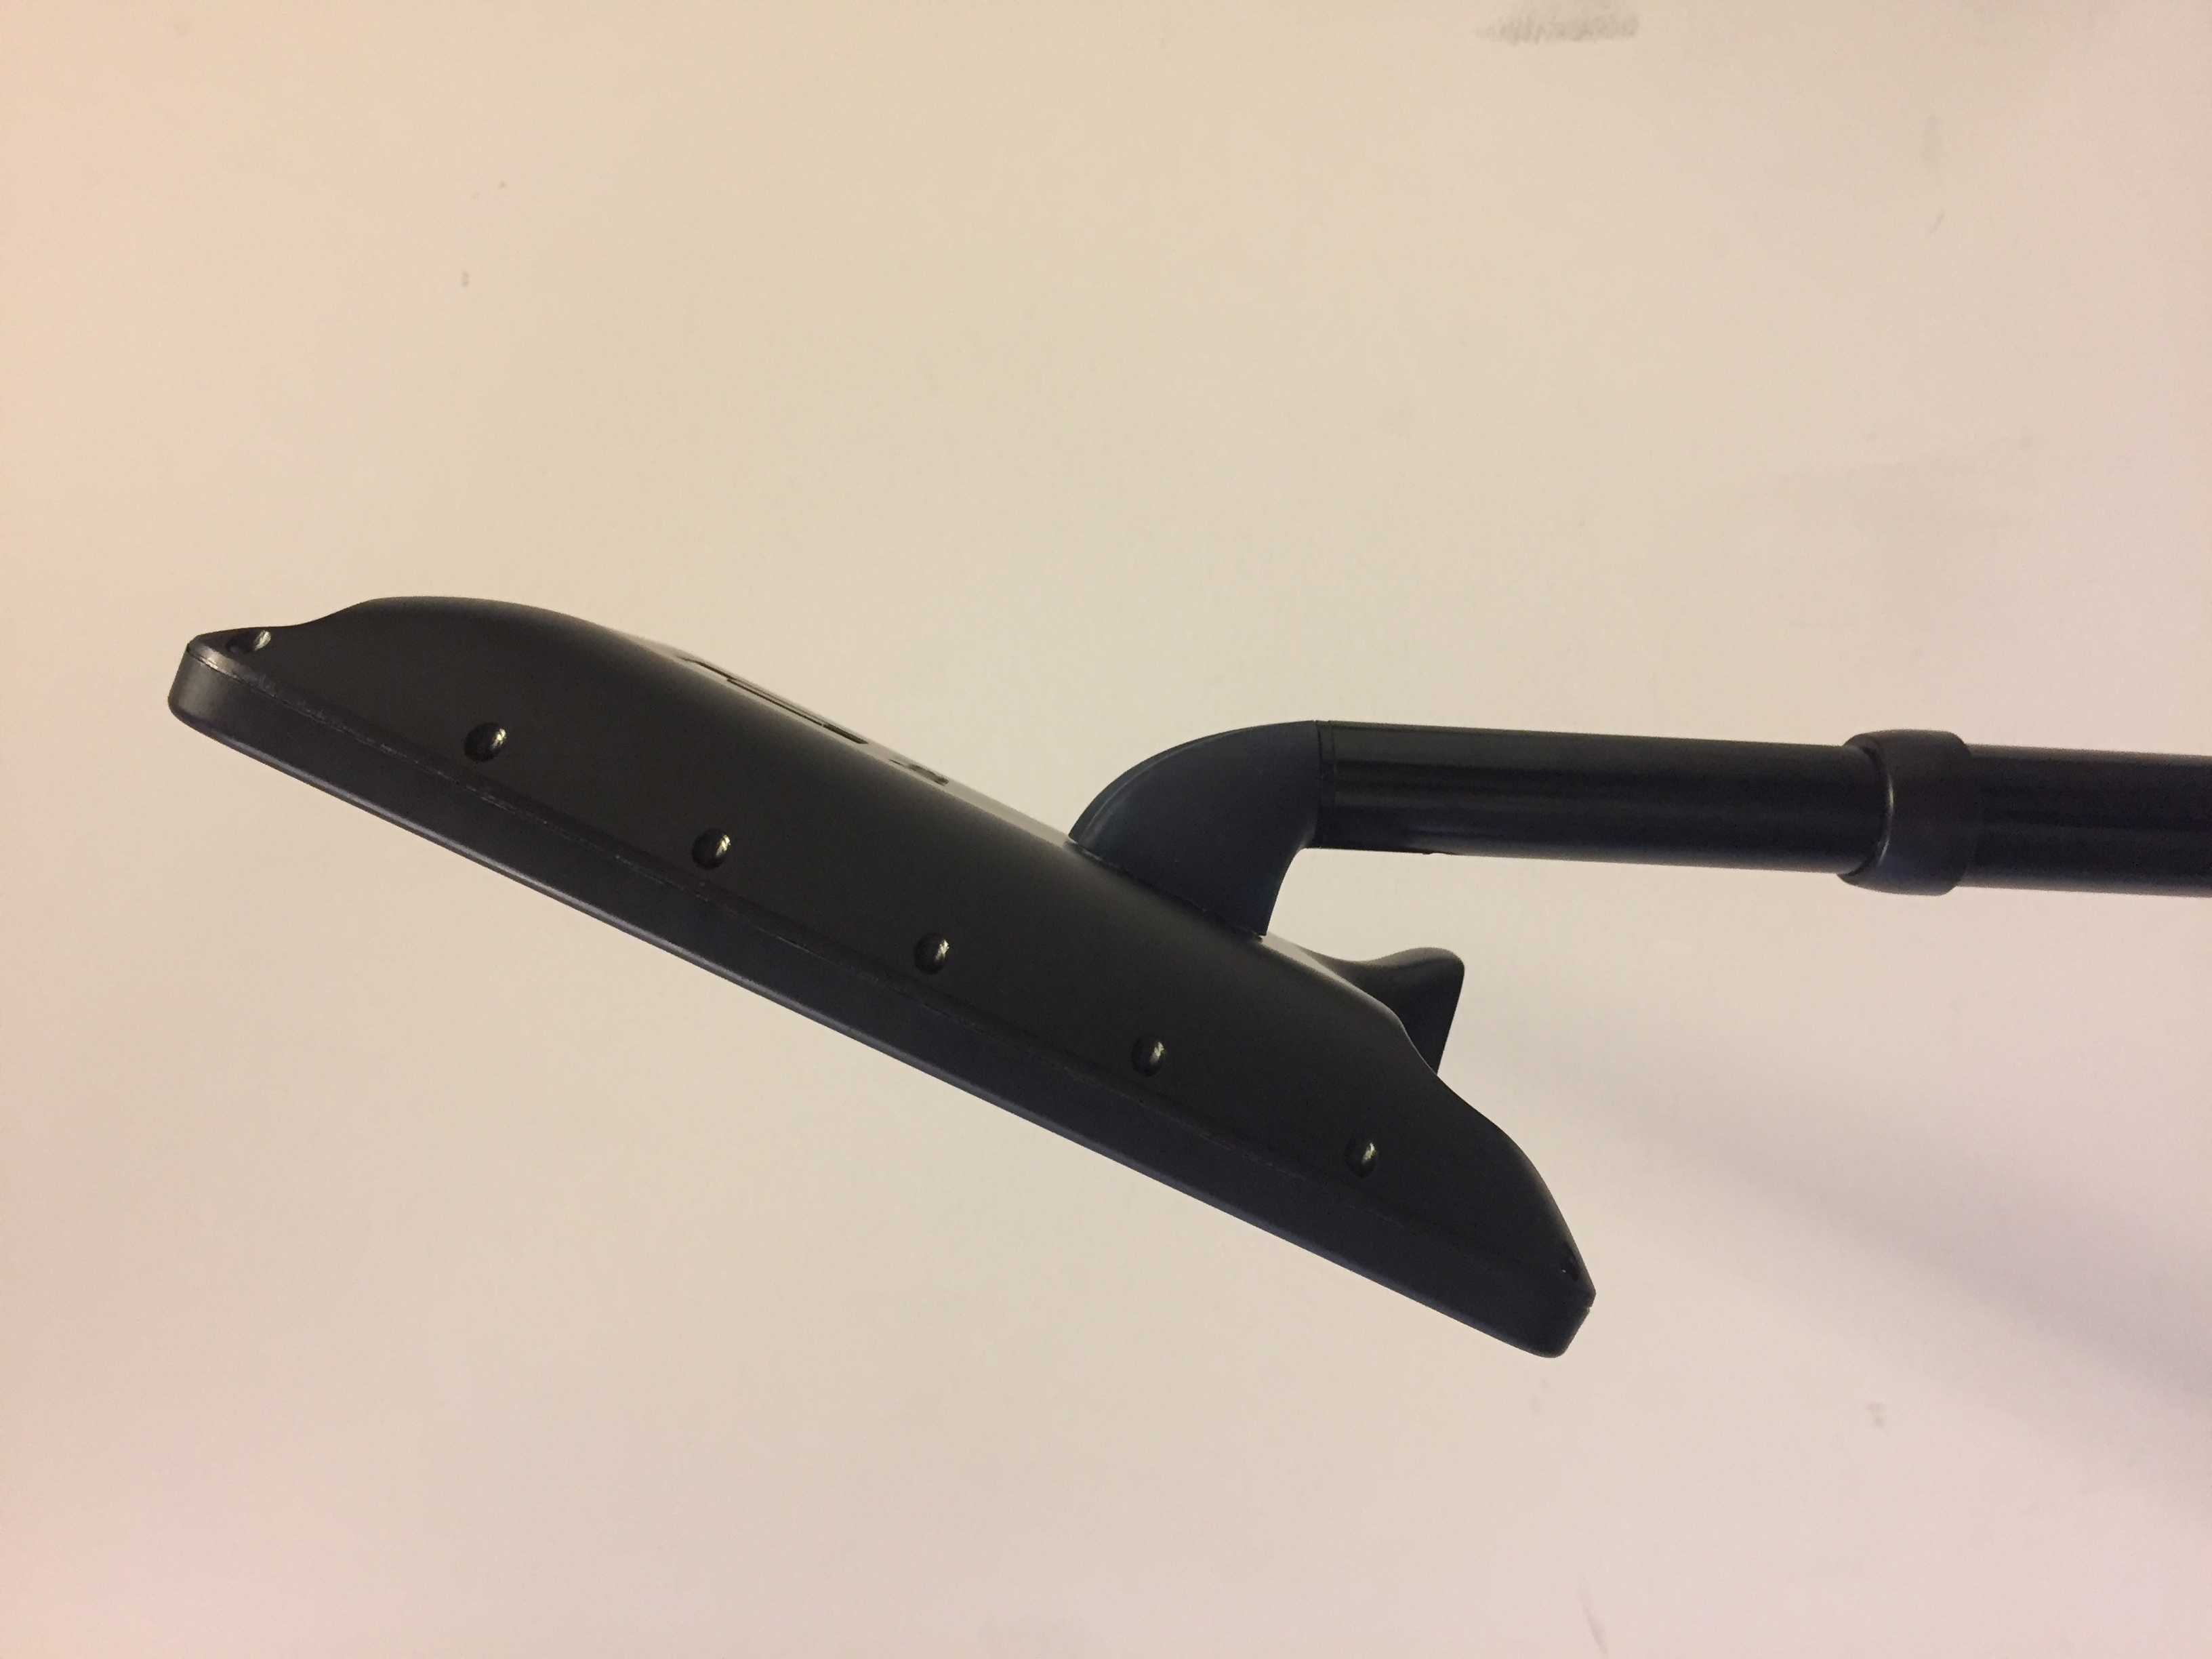
\includegraphics[width=\linewidth, angle =-90]{Figure/ModificeretDoubleSideClose}
  \caption{\textit{Double}'s profile.}
  \label{fig:ModificeretDoubleSideClose}
\end{minipage}
\end{figure}
\noindent
%
%
\begin{figure}[H]
\centering
\includegraphics[width = 0.25\textwidth]{Figure/brug}
\caption{Options presented for the subjects in the interface.}
\label{fig:brug}
\end{figure}
\noindent
% 
\subsection{Semi-structured Interview}
The interview was a two part semi-structured interview. The first part consisted of probing the subjects for their first impression and experience of interacting with the robot in regard to their thoughts about the robot itself and what they think other travellers might think about the interaction. In addition to these conversation topics the subjects were asked about their opinion regarding the robots approach, usefulness, and reliability. Afterwards, the subjects were asked about previous experiences and problems at airports, in order to gather potential use cases where the robot might be helpful. 

%The last topic of conversation in the first part of the interview regards the subjects' previous experiences at an airport, to gather potential use cases for the robot.

%The following are only guidance to the conversation topics and not specific questions:\\ 
%
%\begin{itemize}
%\item First impression of the robot. SKREVET IND
%\item How the robot approached the subject. SKREVET IND
%\item What the subject think about the robot. SKREVET IND
%\item What the subject think other travellers think of their interaction with the robot. SKREVET IN
%\item Robot relevance. SKREVET IND
%\item Robot reliability. SKREVET IND
%\item Experiences at an airport where robot help might have been useful.\\
%\end{itemize}
%\noindent
%
The second part consisted of asking specific questions relating to the robots physical characteristics such as speed, height, distance, movements, appearance, and approach. These questions were asked because these attributes have been found to affect the experience of HRI \cite{PDF:HowMayIServeYou}.\\

The two parts were conducted in continuation of each other and the questions in the second part were only asked if the subjects had not previously answered them spontaneously.
 
\subsection{Roles}
Five researchers were present during the test at AAL. One controlled the \textit{Double} robot, one conducted the interview, and the remaining three observed the travellers as they interacted with or walked past the robot. 

\subsection{Data Processing}
The interviews were transcribed and coded along with observations into affinity notes. The purpose was to create an affinity diagram, which brings insights and issues into a hierarchical diagram based on subjects' statements and behaviour \cite{Wendell2005}. This affinity diagram will be pivotal in eliciting the attributes that affect HRI, and thereafter in creating the scales to be used for further work. To include more of the gathered insigths, it was decided to use both the spontaneous answers from the conversation topics and the answers from the specific questions in the affinity diagram. In total 567 affinity notes were sorted into 10 overall categories with individual subcategories. The 10 superordinate categories were appearance, trust, behaviour, approach, problems with touch screen, avoidance of interaction, personal interest, positivity towards the robot, usefulness, and tech-experience.




%Real travellers were observed interacting with a robot in AAL and interviewed in order to get a sense of peoples' experience and the words they use to describe interacting with a robot in an airport. In total 30 travellers, including 16 women and 14 men, was interviewed during 18 interviews. 11 interviews were performed including a single traveller, where the remaining seven was done on groups of two or more. The participants' ages range from 8 to 62 years (M=37.9, SD=17.1) and have all been travelling more than once.
%
%During the tests a Double robot was used from Double Robotics Inc. Double is basically a segway merged with an iPad and in this study a new head mount was used, so that the iPad was tilted upwards towards the participants, see figure (indsæt billede af double og referencen hertil). Travellers were shown a wireframe on the iPad, intended to help them find a location in the airport of their choosing. In order to create a natural experience, the robot was used to recruit participants by asking them if it could help them find their way around AAL. When travellers were willing to participate the robot led them to the interviewer instead of the chosen gate or restaurant. By doing this, the interviewer could start the interview by asking participants how their first meeting with the robot was without having to first set the scene for the participants and interfering with the natural first impression.
%
%The user experience is then documented like a contextual field study with observations and a semi-structured interview. The interviews are then transcribed and affinity notes are made for building an affinity diagram. By building an affinity diagram these notes can be sorted into a hierarchy of different categories and subcategories, which will tell the user's perspective of the interaction. The affinity diagram represent some of the main areas that are important for travellers when interacting with the robot. These areas are used to create scales, which then are tested with new users in the airport. After gathering data on the chosen parameters, it can then be evaluated in which degree the different attributes contribute to the overall experience of the interaction and how they relate to each other.

\section{Results - Elicitation of attributes}
\label{ResultsElicitation}
%I må gerne tjekke oversættelsen på SQ og labels, så sletter vi de danske SQ efterfølgende og skriver det vigtige
%
In total 567 affinity notes were sorted into 10 overall categories with individual subcategories. The 10 superordinate categories were appearance, trust, behaviour, approach, problems with touch screen, avoidance of interaction, personal interest, positivity towards the robot, usefulness, and tech-experience.

Based on the 10 categories, attributes were elicited according to the criterion of a) being an influencing attribute and b) the possibility of formulating the attributes as a scale question. The field study was conducted on Danish speaking test subjects, and the attributes are therefore listed in both English and Danish. The scale questions are all presented on a \textit{Visual Analoge Scale} (VAS) with closed anchor points and are either bi- or unipolar. If the scale is bipolar a midpoint will be marked either with or without a label. A bipolar scale without a label will be noted with \textit{No label}, whereas an unipolar scale which does not contain a midpoint will be noted with a \textit{-}. 

In the following the 23 derived scales (noted \textit{S}), along with the specific scale question (SQ), will be presented in corresponding order as presented for the test subjects in Experiment 2 and sorted by each page ind the robots interface. An example of each set of scales is given, to illustrate how they were presented in the experiment.
\subsection{Page 1}
\noindent
\textbf{SQ01:} How do think the screen on the robot reacted? \\%(Hvordan synes du, at skærmen på robotten reagerede?)\\
\textbf{SQ02:} How did you experience the robot? \\ %(Hvordan oplevede du robotten?)\\
\textbf{SQ03:} How was it to use the robot?\\% (Hvordan var det at bruge robotten?)\\
\textbf{SQ04}: How did you experience the robot's movements? \\%(Hvordan oplevede du robottens bevægelser?)\\%
See \autoref{tab:ScalesPage1} and \autoref{fig:TilpassetSkaermensReaktion} for how the scales were presented.
\begin{table}[H]
	\centering
\caption{Scale labels PAGE 1}
	\label{tab:ScalesPage1} 
	\begin{tabular}{l|c|c|c}
		S     & Left label & Mid point & Right label \\\hline
		1   & \makecell{Extremely bad\\(Ekstremt dårligt)}  & No label & \makecell{Extremely well \\(Ekstremt godt)}        \\\hline
		2   & \makecell{Extremely unwelcoming \\(Ekstremt afvisende)} & No label & \makecell{Extremely welcoming \\(Ekstremt imødekommende)}         \\\hline
		3   & \makecell{Extremely difficult \\(Ekstremt svært)} & No label & \makecell{Extremely easy \\(Ekstremt nemt)}         \\\hline
	 	4   & \makecell{Extremely wild \\(Ekstremt vilde)} & No label & \makecell{Extremely calm \\(Ekstremt rolige)}               
	\end{tabular}        
\end{table}
\noindent
%
\begin{figure}[H]
\centering
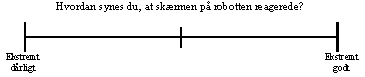
\includegraphics[width = 0.49\textwidth]{Figure/TilpassetSkaermensReaktion}
\setlength\abovecaptionskip{-1.2\baselineskip} 
\caption{Example of a bipolar scale relevant for the scale question: \textit{How do think the screen on the robot reacted?}, rated from \textit{Extremely bad} to \textit{Extremely well}.}
\label{fig:TilpassetSkaermensReaktion}
\end{figure}
\noindent
% 
\subsection{Page 2}
\noindent
\textbf{SQ05:} I think that the robot stopped... \\%(Jeg synes, at robotten stoppede...)\\
\textbf{SQ06:} I think that the robot's speed is... \\%(Jeg synes, at robottens hastighed er...)\\ 
\textbf{SQ07:} I think that the robot's height is... \\%(Jeg synes, at robottens højde er..)\\
See \autoref{tab:ScalesPage2} and \autoref{fig:TilpassetRStoppede} for how the scales were presented on page 2.
\begin{table}[H]
	\centering
\caption{Scale labels PAGE 2}
	\label{tab:ScalesPage2} 
	\begin{tabular}{l|c|c|c}
		S     & Left label & Mid point & Right label \\\hline
		5   & \makecell{Way too close\\(Alt for tæt på)}  & No label & \makecell{Way too far \\(Alt for langt fra)}        \\\hline
		6   & \makecell{Way too slow\\(Alt for langsom)} & \makecell{Fine\\(Fin)} & \makecell{Way too fast \\(Alt for hurtig)}         \\\hline
		7   & \makecell{Way too low \\(Alt for lav)} & \makecell{Fine\\(Fin)} & \makecell{Way too high\\(Alt for høj)}                
	\end{tabular}        
\end{table}
\noindent
%
\begin{figure}[H]
\centering
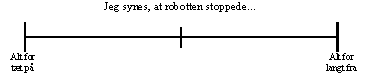
\includegraphics[width = 0.49\textwidth]{Figure/TilpassetRStoppede}
\setlength\abovecaptionskip{-1.2\baselineskip} 
\caption{Example of a bipolar scale relevant for the scale question: \textit{I think that the robot stopped...}, rated from \textit{Way too close} to \textit{Way too far}.}
\label{fig:TilpassetRStoppede}
\end{figure}
\noindent
% 
\subsection{Page 3 and 4}
\noindent
\textbf{SQ08:} I feel that the robot can help me\\% (Jeg føler, at robotten kan hjælpe mig)\\
\textbf{SQ09}: I think that the robot was obstructing me\\%(Jeg synes, at robotten stod i vejen)\\
\textbf{SQ10:} I feel safe around the robot\\%(Jeg føler mig tryg ved robotten)\\
\textbf{SQ11:} The robot startled me\\ %(Robotten gjorde mig forskrækket)\\
\textbf{SQ12:} I like to be served by the robot\\% (Jeg kan godt lide at blive betjent af robotten)\\
\textbf{SQ13:} I counted on the robot to lead me to the location I chose\\% (Jeg regnede med, at robotten fulgte mig hen til det sted jeg valgte)\\
See \autoref{tab:ScalesPage3} and  \autoref{fig:TilpassetRobottenKanHjaelpe} for how the scales were presented on page 3 and 4.
\begin{table}[H]
	\centering
\caption{Scale labels PAGE 3 and 4}
	\label{tab:ScalesPage3} 
	\begin{tabular}{l|c|c|c}
		S     & Left label & Mid point & Right label \\\hline
		8-13   & \makecell{Completely disagree\\(Helt uenig)}  & No label & \makecell{Completely agree\\(Helt enig)}                      
	\end{tabular}        
\end{table}
\noindent
%
\begin{figure}[H]
\centering
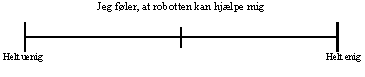
\includegraphics[width = 0.49\textwidth]{Figure/TilpassetRobottenKanHjaelpe}
\setlength\abovecaptionskip{-1.9\baselineskip} 
\caption{Example of a bipolar scale relevant for the scale question: \textit{I feel that the robot can help me}, rated from \textit{Completely disagree} to \textit{Completely agree}.}
\label{fig:TilpassetRobottenKanHjaelpe}
\end{figure}
\noindent
% 
\subsection{Page 5}
\noindent
\textbf{SQ14:} How personal did you experience the robot's help?\\% (Hvor personlig oplevede du robottens hjælp?)\\
\textbf{SQ15:} How surprised were you by the robot's approach?\\% (Hvor overrasket blev du over robottens henvendelse?)\\
For each of the two scale questions the chosen labels are listed in \autoref{tab:ScalesPage5}. Also see \autoref{fig:TilpassetPersonligHjaelp} for an example of the scale used.
%
\begin{table}[H]
	\centering
\caption{Scale labels PAGE 5}
	\label{tab:ScalesPage5} 
	\begin{tabular}{l|c|c|c}
		S     & Left label & Mid point & Right label \\\hline
		14   & \makecell{Not at all personal\\(Slet ikke personlig)}  & - & \makecell{Extremely personal\\(Ekstremt personlig)}        \\\hline
		15   & \makecell{Not at all surprised\\(Slet ikke overrasket)} & - & \makecell{Extremely surprised \\(Ekstremt overrasket)}               
	\end{tabular}        
\end{table}
\noindent
%
\begin{figure}[H]
\centering
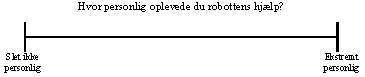
\includegraphics[width = 0.49\textwidth]{Figure/TilpassetPersonligHjaelp}
\setlength\abovecaptionskip{-1.2\baselineskip} 
\caption{Example of an unipolar scale relevant for the scale question: \textit{How personal did you experience the robots help?}, rated from \textit{Not at all personal} to \textit{Extremely personal}.}
\label{fig:TilpassetPersonligHjaelp}
\end{figure}
\noindent
% 
\subsection{Page 6}
\noindent
\textbf{Q:} What do you think about the robot?\\% (Hvad synes du om robotten)\\
This question covers scales 16-19. The scale used was similar to that shown in \autoref{fig:TilpassetPersonligHjaelp}. See \autoref{tab:ScalesPage6} for the labels used.
%
\begin{table}[H]
	\centering
\caption{Scale labels PAGE 6}
	\label{tab:ScalesPage6} 
	\begin{tabular}{l|c|c|c}
		S     & Left label & Mid point & Right label \\\hline
		16   & \makecell{Not at all annoying\\(Slet ikke irriterende)}  & - & \makecell{Extremely annoying \\(Ekstremt irriterende)}        \\\hline
		17   & \makecell{Not at all elegant \\(Slet ikke elegant)} & - & \makecell{Extremely elegant \\(Ekstremt elegant)}         \\\hline
		18   & \makecell{Not at all exciting\\(Slet ikke spændende)} & - & \makecell{Extremely exciting \\(Ekstremt spændende)}         \\\hline
	 	19   & \makecell{Not at all cute\\(Slet ikke sød)} & - & \makecell{Extremely cute \\(Ekstremt sød)}               
	\end{tabular}        
\end{table}
\noindent
%
\subsection{Page 7}
\noindent
\textbf{Q:} What else do you think about the robot?\\%(Hvad synes du ellers om robotten?)\\
This question covers scales 20-23. The scale used was similar to that shown in \autoref{fig:TilpassetPersonligHjaelp}. See \autoref{tab:ScalesPage7}.
%
\begin{table}[H]
	\centering
\caption{Scale labels PAGE 7}
	\label{tab:ScalesPage7} 
	\begin{tabular}{l|c|c|c}
		S    & Left label & Mid point & Right label \\\hline
		20   & \makecell{Not at all cool\\(Slet ikke sej)}  & - & \makecell{Extremely cool \\(Ekstremt sej)}        \\\hline
		21   & \makecell{Not at all intrusive \\(Slet ikke anmassende)} & - & \makecell{Extremely intrusive \\(Ekstremt anmassende)}         \\\hline
		22   & \makecell{Not at all funny\\(Slet ikke sjov)} & - & \makecell{Extremely funny \\(Ekstremt fun)}         \\\hline
	 	23   & \makecell{Not at all human \\(Slet ikke menneskelig)} & - & \makecell{Extremely human \\(Ekstremt menneskelig)}               
	\end{tabular}        
\end{table}
\noindent
%
Based on the affinity diagram a 24th attribute was derived, this attribute will not be presented along side the aforementioned scales but will be included in a separate demographic page as it does not directly concern the robot. The attribute is formulated in the scale question: \textit{How fond of technology are you?}, which will be evaluated on an unipolar scale, similar to the other unipolar scales, with anchor points: \textit{Not at all fond} (slet ikke glad) and \textit{Extremely fond} (ekstremt glad).\\  

\noindent
When comparing the attributes for HRI found in this study with attributes for HRI from previous conducted studies on social robots \cite{PDF:ExploringInfluencingVariable}, \cite{PDF:SharingALifeHarvey}, \cite{PDF:InTheCompanyofRobots}, \cite{PDF:CloseButNotStuck}, \cite{PDF:TheImpactOfTraveler}, \cite{PDF:HumanRobotEmodiedInteraction}, \cite{PDF:RecommendationEffects}, attributes such as distance, anthropomorphism, height, speed, movement, trust, enjoyment, technological knowledge, and usefulness reoccur. New attributes were found compared with previous mentioned studies these are: Elegance, cute, cool, startled, exciting, welcoming, obstructive, robot help as personal, and wether the encounter with the robot was surprising. However, these might be measured indirectly in the aforementioned studies.

Accordring to \cite{PDF:HowSocialDistanceShapesHRI} \textit{social distance} has an effect on HRI. Even though the subjects in AAL did not mention it specifically it seems that this is due to \textit{power distance}, where the subjects feel in control as they were the dominant part and the robot was the subordinate in the interaction. Furthermore this could also be due to the given HRI task was cooperative as the robot's purpose was to help the subject to a specific location of their choosing. When focusing on \textit{task distance} when in cooperative tasks it seems as if the subjects acted more friendly, intimate, and involved in the interaction with the robot, which is based on all the positive comments from subjects \fxnote{Jeg forstår ikke denne sætning. Måske en omskrivning? - Korn.}
 
  





\section{Part II - Scale Testing}
\label{MethodScaleTesting}
%{\color{red} Metoden for anden test beskrives i dette afsnit. Hvis der er gentagelser ift første test vil der blot laves en henvisning til det forrige metode afsnit}
This section describes the second part of the study where the scales were tested at AAL. The purpose was to get the travellers to rate their experience with the interaction on the developed scales. Afterwards the results might show if any scales are redundant or needs to be reformulated.
%

\section{Method}
\label{Method2}
The test was conducted over the course of two days and otherwise as described in \autoref{MethodElicitation}. The location stayed the same along with the overall procedure. This time, instead of being led to an interview by the robot, the subjects were led a small distance in the direction of Duty Free where most of the available options in the wireframe were (Food, Shopping, Gates). Here an experimenter politely stopped them and informed them about the ongoing study. After they accepted to participate, they were led to a PC nearby to rate their experience on the developed scales. The experimenter was ready to take notes while they rated. The order in which the scales were presented is described in \autoref{ResultsElicitation}. The physical parameters of the robot were varied over the course of the test. This included: the angle of approach, the robot height (and speed), and the distance to the participant. As a consequence of the study being ecologically performed in an actual airport it was not possible to precisely control the distance to the participant or the angle of approach. These had to rely on subjective judgement on the researchers part. Height was measured using a measuring tape.

\subsection{Materials}
The same materials were used as described in \autoref{MethodElicitation} along with the same \textit{Double} and tilted headmount. Additionally, software was developed in Processing (\url{www.processing.org}) to be able to collect data from the scales. The program was presented on a \textit{Microsoft Surface Pro (5)} with a simple wireless mouse. The 24th scale was presented on a sheet of paper along with a few questions to collect demographic information.

\subsection{Scale Program}
The scale program consisted of 23 scales distributed on 7 pages. The number of scales presented on a single page were maximum four and minimum two. The subjects were instructed to set a fitting marker on the scales using the provided mouse. The scales were organised to be as consistent on each page as possible e.g. the same type of scales with a mid-point were presented on one page.

\subsection{Subject Recruitment}
Over the course of two days 43 subjects participated. They were aged from 10 to 72 (M=40.1, SD=13.4) and distributed among 16 females and 27 males. Subjects reported that they travel between 1 and 100 times per year (M=15.3, SD=18.1). The subjects were again recruited by the robot with the same wireframe as in the previous test.

\subsection{Roles}
Four researchers were present during the test at AAL. One controlled the \textit{Double} robot, one instructed the subjects to answer the scales, one observed when the robot should start leading the subjects towards Duty Free and one noted the physical parameters of the robot such as height, direction of approach and distance to the subjects.

\subsection{Data Processing}
Data was gathered via the scale program for each participant in a .csv format and analysed using both Matlab and R. It was analysed using multivariate Principal Component Analysis (PCA) and boxplots on the overall data. The subjects were generally categorised in three groups (three groups within age, height ratio, distance, direction etc.) in order to assess how the participants responded to the physical changes of the robot \fxnote{rettes til}.

%\subsection{Materials}
%\label{MaterialsScaleTesting}
%%
%The same \textit{Double} robot with the same headmount and wireframe was used in this test. Besides that a \textit{Microsoft Surface Pro (5)} computer was used to show and collect answers from the 23 scales. To collect demographic information a sheet of paper with a few questions was used.
%\subsection{Subject Recruitment}
%43 subjects from the age of 10 to 72 years (M=40.1, SD=13.4) distributed among 16 females and 27 males participated. The subjects were recruited with the same procedure and with the same questions in this test as in the previous. 
%\subsection{Roles}
%Four researchers were present during the test at AAL. One controlled the \textit{Double} robot, one got the subjects to answer on the scales, one kept an eye on when the robot should start leading the subjects towards duty free and one noted the physical parameters of the robot.
%\subsection{{\color{red}Data Processing}}


\section{Results - Scale Testing}
\label{ResultsScaleTesting}
%
Due to a programming error the dataset contains several zero-answers which could happen when subjects did not answer on a scale. It was decided to remove the missing answers. Two criteria were used to determine when to exclude some of the zero-points that occurred because of a non-answered scale. 1) If all scale ratings presented on one of the pages are zero, it was probably because subjects skipped a page and 2) If there is a strong tendency for high ratings on a scale and a single zero-answer seems unlikely, it was denoted as a missing answer.\\

\noindent
The different ratings on the scales in the second test are visualised on \autoref{fig:Boxplot}.
%
%\begin{figure}[H]
%	\centering
%	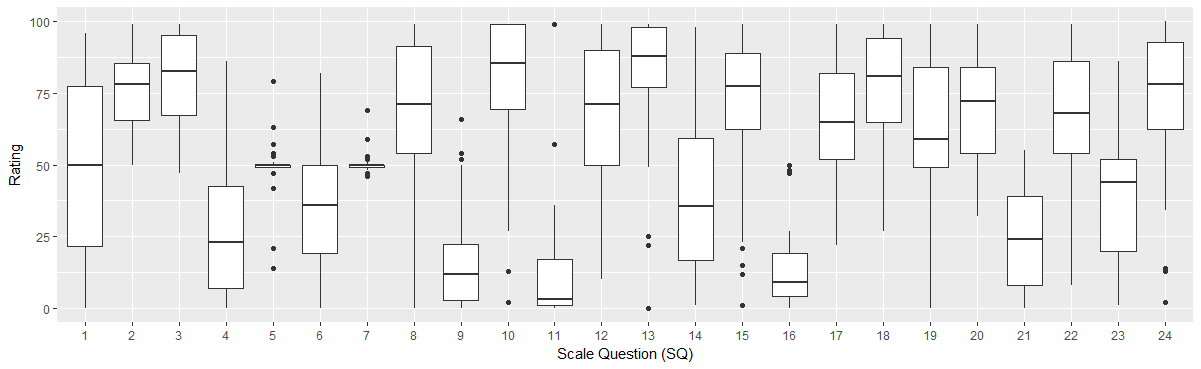
\includegraphics[width = 0.49\textwidth]{Figure/Boksplot24uden0}
%	\setlength\abovecaptionskip{-1.2\baselineskip} 
%	\caption{Boxplot showing the 24 attributes. The boxplot shows the median, where the box is ranging from 25-75 \% of the data, and the whiskers from 0-25 \% and 25-100 \% of the data.}
%	\label{fig:Boxplot}
%\end{figure}
%\noindent
%

\begin{figure*}[!b]
	\centering
	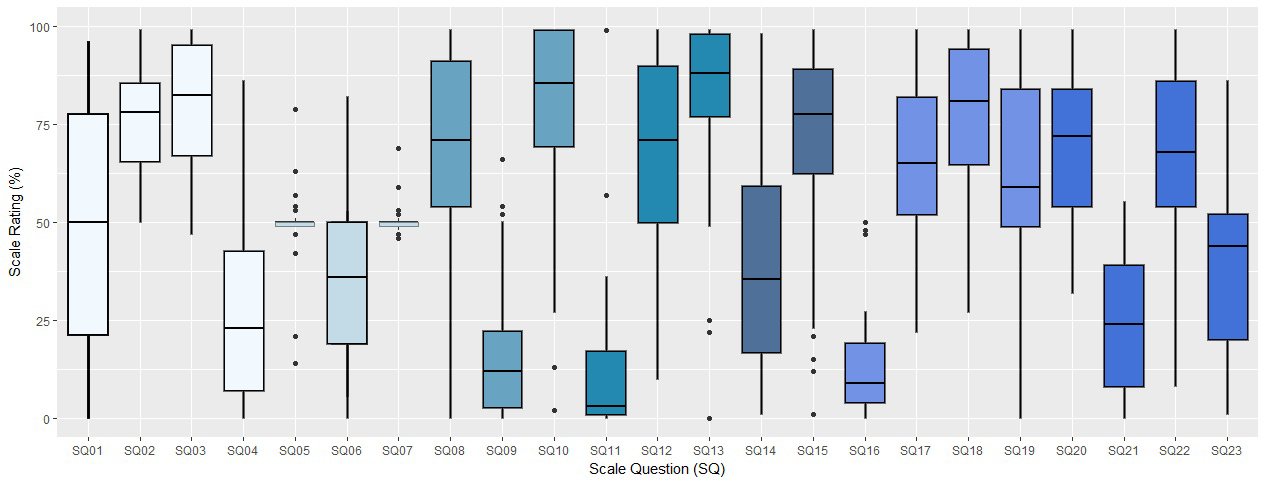
\includegraphics[width=6.9in]{Figure/Boksplot23.png}
	\hfil
%	\subfloat[]{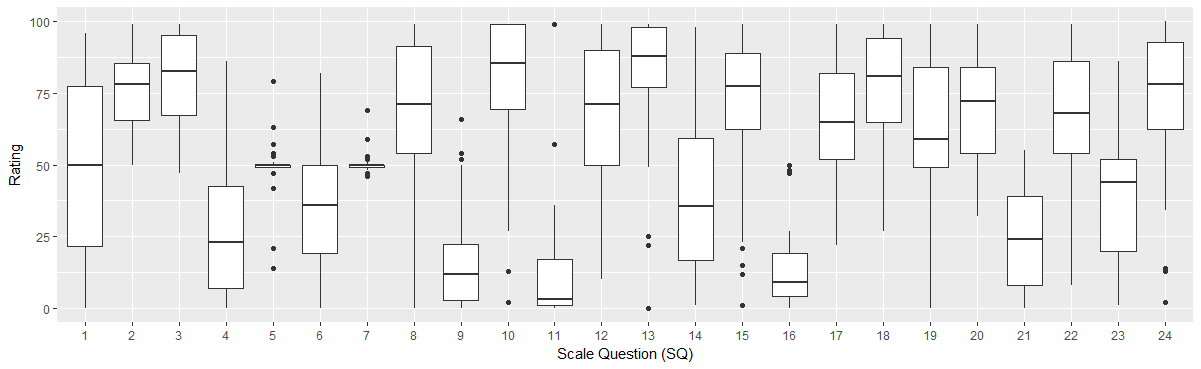
\includegraphics[width=2.5in]{Figure/Boksplot24uden0}
%		\label{fig_second_case}}
	\caption{Boxplot showing the 23 attributes. The boxplot shows the median, where the box is ranging from 25-75 \% of the data, and the whiskers from 0-25 \% and 75-100 \% of the data. Each colour represents a new page of scales.}
	\label{fig:Boxplot}	
\end{figure*}
%
From \autoref{fig:Boxplot} it is notable that there exists much greater variation in some scales compared to others. For some SQs, a big part of the scale is used (1, 4, 8, 12, 14, 19), where for others a smaller part of the scale is used (2, 3, 5, 7, 9, 11, 13, 16). Furthermore some of the scale ratings appears normal distributed (1, 2, 6, 17, 20, 21) and others appears skewed (8, 9, 10, 11, 13, 18). In some SQs the data accumulates around midpoints or anchor points (5, 7, 9, 10, 11, 13, 16). SQ05 and SQ07 are centralised around the midpoint, which for SQ07 can relate to the label \textit{fine} being too broadly describing. The closed anchor points used on the scales can induce accumulation of data points around these. Also the use of bipolar scales poses the risk of picking two words which are not  each others opposite.

When looking at gender differences it seems that women rated SQ04, SQ11, and SQ21 lower than men. It suggests that females experienced the movements of the robot more calm compared to males, but also that they find the robot less intrusive and startling.\\
When conducting a PCA on all the scale results it showed that only 53.1 \% of the total variance is explained when using the first three dimensions, which is why PCA relating to different groups such as the robot's height, distance, and direction are conducted in order to reduce the dimensions and to be able to explain more of the variance. Figure~\ref{fig:Scree} shows a Scree plot from PCA relating to the robot's height, where 94.1 \% of the variance is explained using three dimensions. Figure~\ref{fig:biplot} shows the Biplot relating to the robot's height. Similar Biplots were made for direction and distance. The attributes which loads the most on the components are:

\noindent
\textbf{Height:} SQ19 appears to contribute the most to PC1. SQ01 the most to PC2. SQ06 the most to PC3. \\
\textbf{Distance:} SQ01 appears to contribute the most to PC1 along with SQ15. SQ10 contributes most to PC2.\\
\textbf{Direction:} SQ10 contributes most to PC1. SQ22 and SQ23 contributes almost equally to PC2. SQ13 and SQ20 contributes almost equally to PC3.\\
%


\begin{figure*}[!t]
\centering
\subfloat[Scree Plot of Robot]{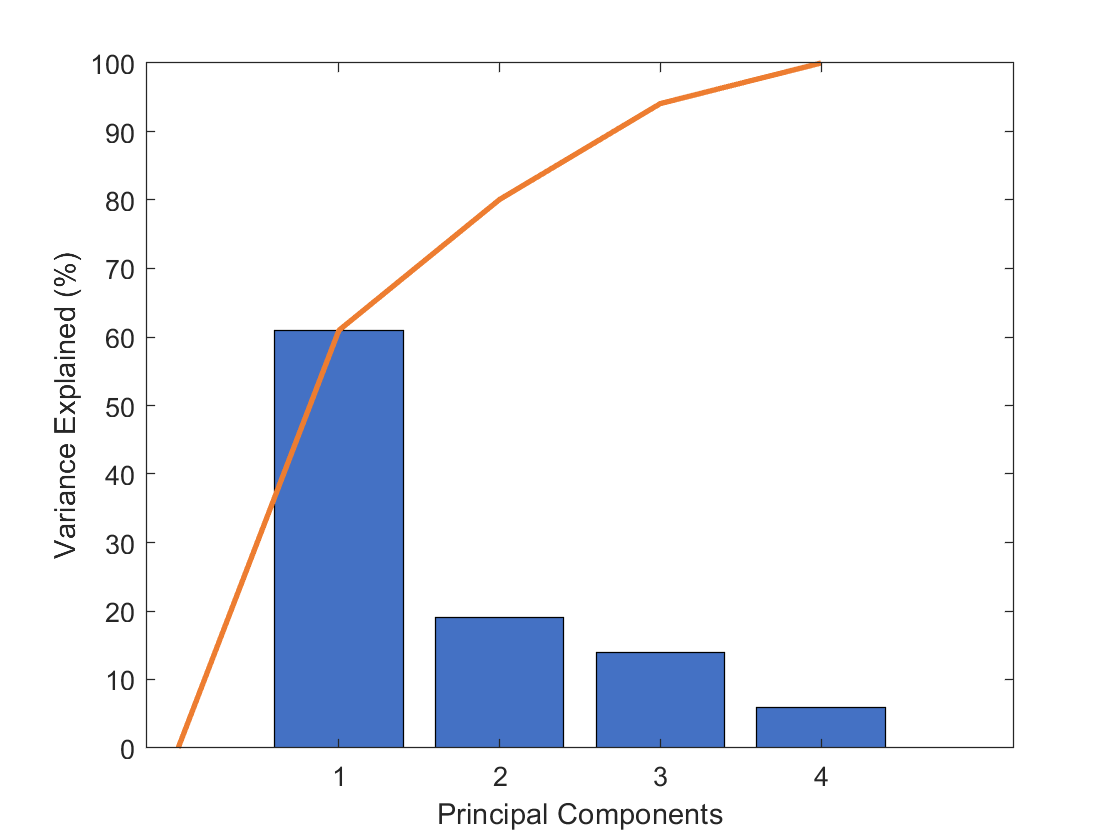
\includegraphics[width=2.5in]{Figure/Scree.png}
\label{fig_first_case}}
\hfil
\subfloat[Biplot of Robot Height]{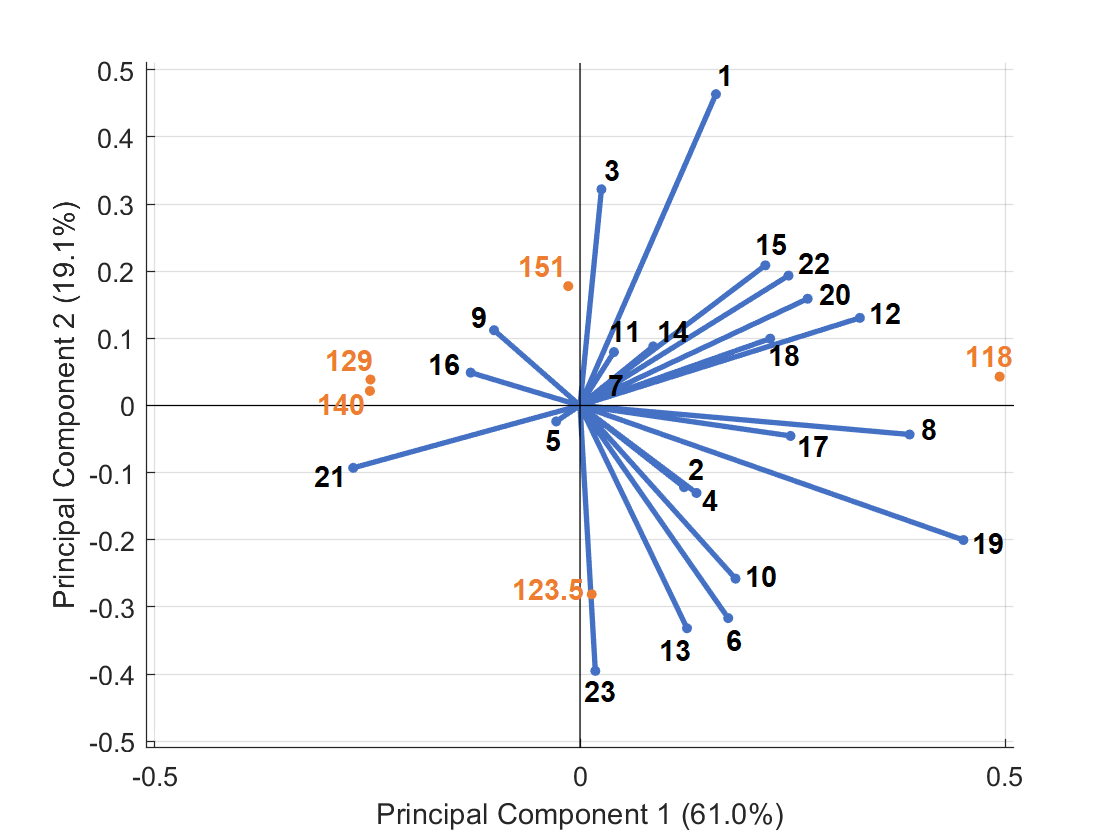
\includegraphics[width=2.5in]{Figure/RHeight-Biplot.png}
\label{fig_second_case}}
\caption{\textbf{(a):} Scree plot showing the connection between the number of Principal Components and Variance Explained (\%): PC1 (61 \%), PC2 (19.1 \%), PC3(14 \%), PC4(5.9 \%). \textbf{(b):} Biplot showing how the different attributes contributes to components and which attributes that correlates. The black numbers denotes SQ and the red to the different heights in cm.}
\label{fig_sim}
\end{figure*}
%******
%\begin{figure*}[!t]
%\centering
%\subfloat[Case I]{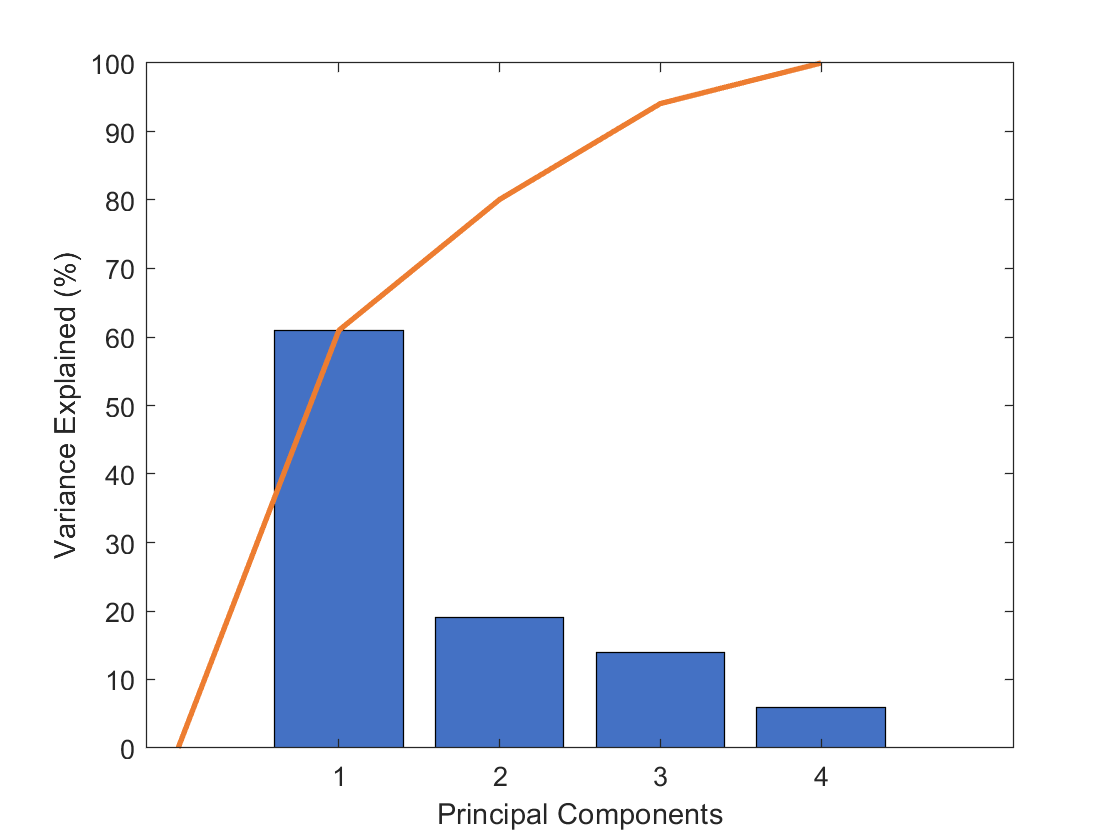
\includegraphics[width=2.5in]{Figure/Scree.png}
%\label{fig_first_case}}
%\hfil
%\subfloat[Case II]{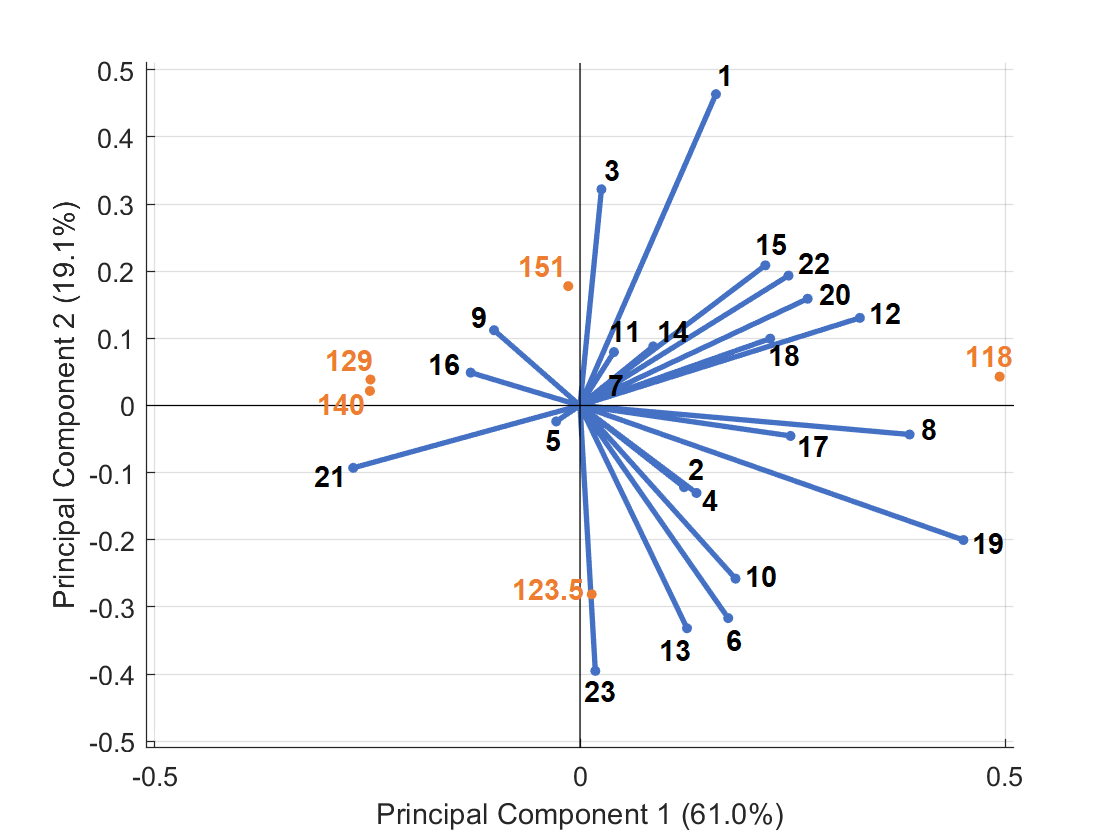
\includegraphics[width=2.5in]{Figure/RHeight-Biplot.png}
%\label{fig_second_case}}
%\caption{}
%\label{fig_sim}
%\end{figure*}
%***********************
%\begin{figure}[!b]
%\centering
%\begin{minipage}{0.25\textwidth}
%  \centering
%  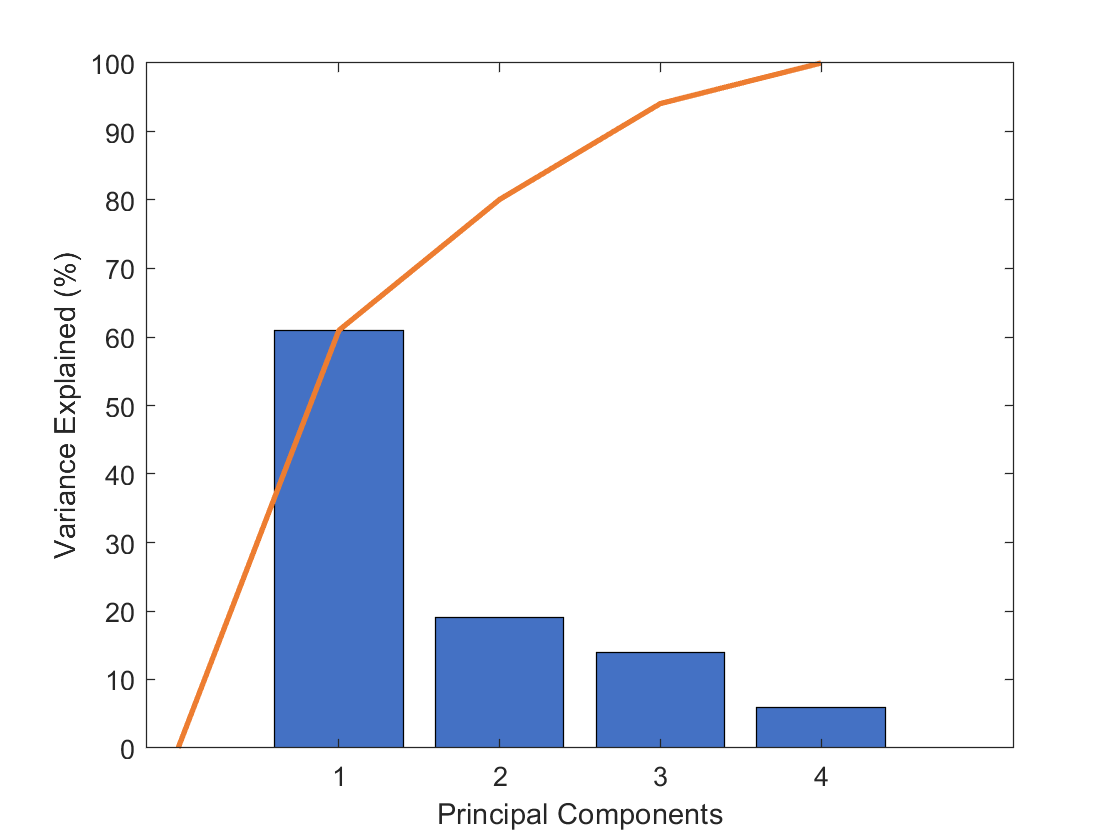
\includegraphics[width =\textwidth]{Figure/Scree.png}
%  \caption{\textit{Double}'s front.}
%  \label{fig:ModificeretDoubleFront}
%\end{minipage}%
%\begin{minipage}{0.25\textwidth}
%  \centering
%	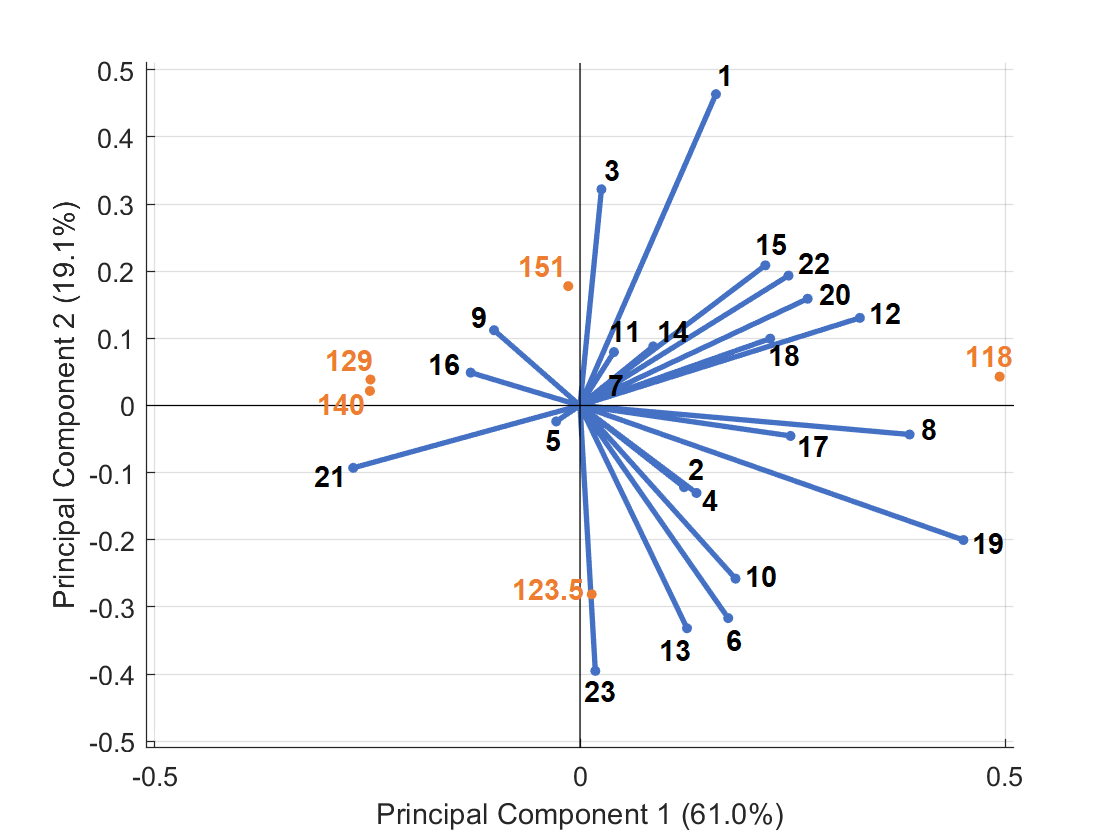
\includegraphics[width = \textwidth]{Figure/RHeight-Biplot.png}
%  \caption{\textit{Double}'s profile.}
%  \label{fig:ModificeretDoubleSideClose}
%\end{minipage}
%\end{figure}
%\begin{figure}[H]
%	\centering
%	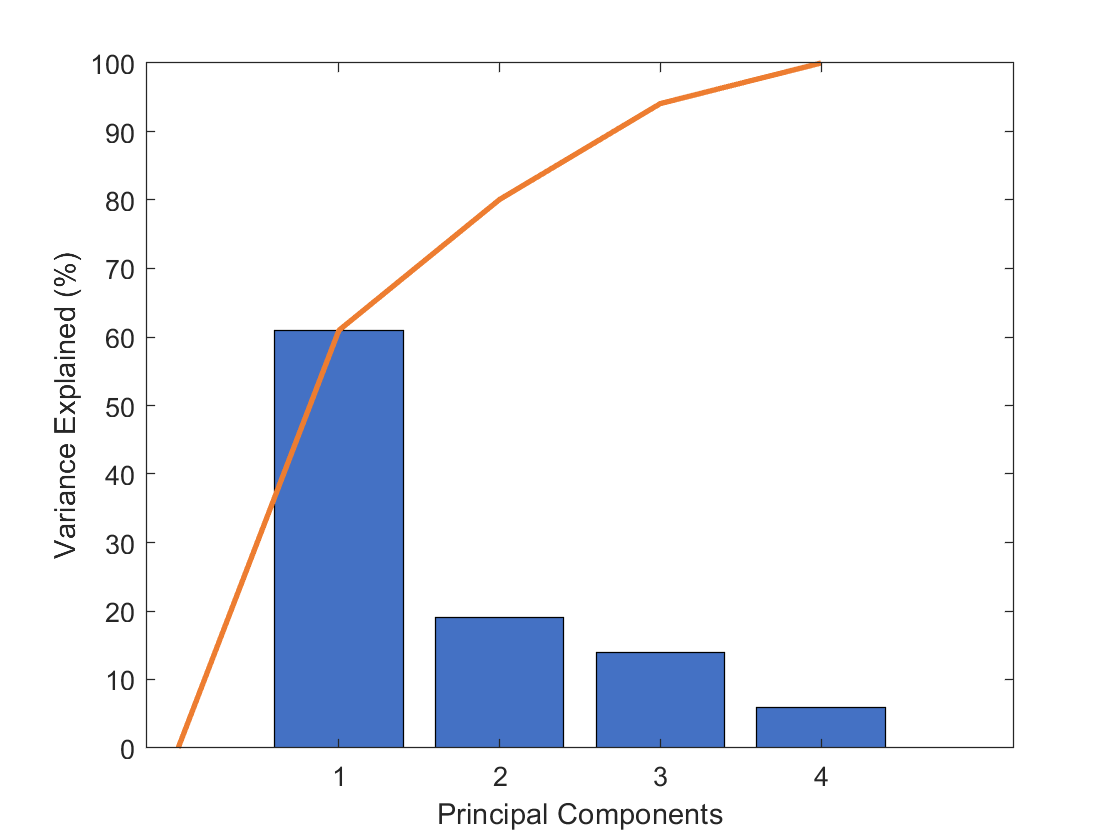
\includegraphics[width = 0.40\textwidth]{Figure/Scree.png}
%	\caption{Scree plot showing the connection between the number of Principal Components and Variance Explained (\%): PC1 (61 \%), PC2 (19.1 \%), PC3(14 \%), PC4(5.9 \%).}
%	\label{fig:Scree}
%\end{figure}
%\noindent
%%
%\begin{figure}[H]
%	\centering
%	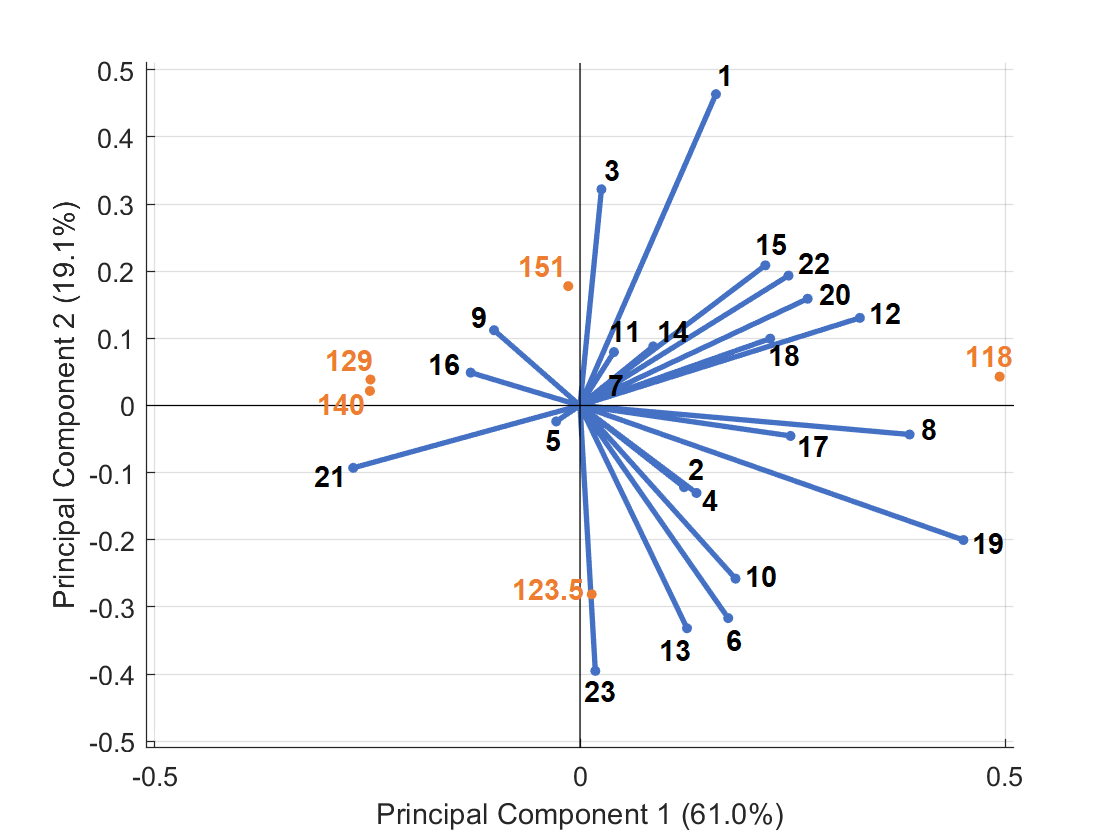
\includegraphics[width = 0.40\textwidth]{Figure/RHeight-Biplot.png}
%	\caption{Biplot showing how the different attributes contributes to components and which attributes that correlates. The black numbers denotes SQ and the red to the different heights in cm.}
%	\label{fig:biplot}
%\end{figure}
%\noindent
%
2D and 3D Biplots from the different PCAs shows positive and negative correlations between different attributes. These correlations are presented in \autoref{tab:CorrelationsFromPCA}.
%
\begin{table}[H]
	\centering
	\caption{Correlations from PCA}
	\label{tab:CorrelationsFromPCA} 
	\begin{tabular}{ c|c|c }
		\centering
		PCA & Positive correlation & Negative correlation \\ \hline
		\multirow{5}{*}{Height} & SQ08  + SQ17 & SQ02  + SQ09 \\
		& SQ10 + SQ13 & SQ04 + SQ12 \\
		& SQ12 + SQ18 & SQ12 + SQ21 \\
		& SQ14 + SQ15 & SQ16 + SQ19 \\
		& SQ20 + SQ22 & SQ18 + SQ21\\ \hline
		\multirow{6}{*}{Distance} & SQ01 + SQ12 & SQ02 + SQ09 \\
		& SQ07 + SQ17 & SQ05 + SQ21 \\
		& SQ08 + SQ21 & SQ10 + SQ13 \\
		& SQ10 + SQ22 & SQ13 + SQ22 \\
		&  & SQ14 + SQ16 \\	
		&  & SQ19 + SQ20 \\ \hline	
		\multirow{5}{*}{Direction} 
		& SQ05 + SQ07 & SQ01 + SQ12 \\
		& SQ08 + SQ10 & SQ06 + SQ23 \\
		& SQ09 + SQ14 & SQ09 + SQ10 \\
		& SQ18 + SQ20 & SQ10 + SQ14 \\
		&  & SQ13 + SQ21
	\end{tabular}        
\end{table}
\noindent
%
To investigate these correlations further, ratings from correlating SQs are compared, as seen in \autoref{fig:SQ12+SQ18}. Even though correlations occur when doing PCA on groupings, these plots of comparison do not take groupings into consideration. This might be why some correlations are not found when comparing SQs, even though the Biplots showed a correlation. From \autoref{fig:SQ12+SQ18} it can be seen that the robot is perceived more exciting when subjects like to be served by the robot. Attributes that have a clear correlation from this kind of comparison are shown in \autoref{tab:CorrelationsFromGraphs}.
%
\begin{figure}[H]
	\centering
	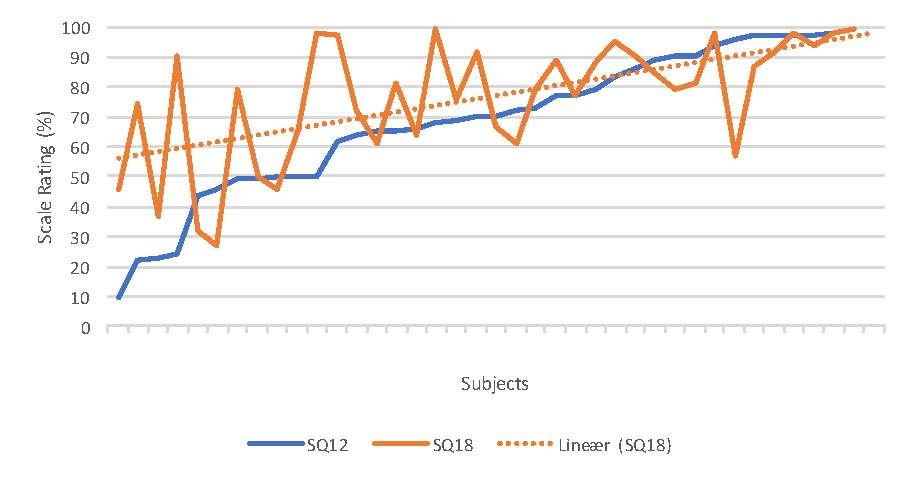
\includegraphics[width = 0.49\textwidth]{Figure/SQ12+SQ18}
	\setlength\abovecaptionskip{-1.2\baselineskip} 
	\caption{Comparison between ratings on SQ12 and SQ18 based on 41 subjects. Two were removed due to incomplete datasets.}
	\label{fig:SQ12+SQ18}
\end{figure}
\noindent
%
\begin{table}
	\centering
	\caption{Correlations from graphs}
	\label{tab:CorrelationsFromGraphs} 
	\begin{tabular}{ c|c }
		\centering
		Positive correlation & Negative correlation \\ \hline
		SQ04 + SQ09 & SQ02 + SQ09 \\ 
		SQ08 + SQ10 & SQ09 + SQ10 \\ 
		SQ08 + SQ17 & SQ12 + SQ21 \\ 
		SQ10 + SQ13 & SQ13 + SQ21 \\ 
		SQ12 + SQ18 & SQ18 + SQ21	\\	
		SQ18 + SQ20 & 			\\
		SQ20 + SQ22 & 
	\end{tabular}        
\end{table}
\noindent
%
The physical variables can be compared with SQs as well as the demographic parameters in the same manner as comparing SQs with each other, to see how these variables and parameters affect the ratings of the attributes. \autoref{fig:HeightSQ6} were SQ06 is compared with the robot's height shows that when the robot's height increases the robot is perceived as being less annoying. When comparing SQ06 with age, the younger a subject is, the more inclined one is to rate the robot as moving too slow. Also, a small negative correlation was noted in relation to how exciting and funny the robot seemed. The older the subjects were, the less exciting and funny they rated the robot. Within height the smaller the robot was the faster and more wild it was rated. This was expected, as the robot automatically moves more slowly when the height increases and faster when the height decreases. Additionally it was rated more cute, elegant, and trustworthy, regarding to wayfinding, when it was small.
%
\begin{figure}[H]
	\centering
	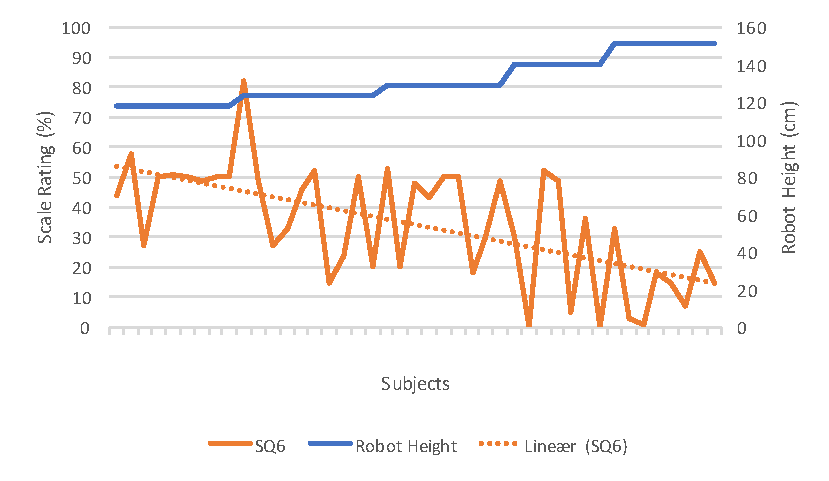
\includegraphics[width = 0.49\textwidth]{Figure/HeightSQ6}
	\setlength\abovecaptionskip{-1.2\baselineskip} 
	\caption{Comparison between the robot's five heights (cm) and ratings (\%) on SQ06 based on all subjects.}
	\label{fig:HeightSQ6}
\end{figure}
\noindent
%

%\section{Part II}
This section will describe the second part of the study where the scales were tested at AAL and in the same location as before. The purpose was to get the travellers to rate their experience with their interaction on the developed scales. Afterwards the results might show if any scales are redundant or needs to be reformulated.




\section{Method}
\label{Method2}
The test was conducted over the course of two days and otherwise as described in \autoref{MethodElicitation}. The location stayed the same along with the overall procedure. This time, instead of being led to an interview by the robot, the subjects were led a small distance in the direction of Duty Free where most of the available options in the wireframe were (Food, Shopping, Gates). Here an experimenter politely stopped them and informed them about the ongoing study. After they accepted to participate, they were led to a PC nearby to rate their experience on the developed scales. The experimenter was ready to take notes while they rated. The order in which the scales were presented is described in \autoref{ResultsElicitation}. The physical parameters of the robot were varied over the course of the test. This included: the angle of approach, the robot height (and speed), and the distance to the participant. As a consequence of the study being ecologically performed in an actual airport it was not possible to precisely control the distance to the participant or the angle of approach. These had to rely on subjective judgement on the researchers part. Height was measured using a measuring tape.

\subsection{Materials}
The same materials were used as described in \autoref{MethodElicitation} along with the same \textit{Double} and tilted headmount. Additionally, software was developed in Processing (\url{www.processing.org}) to be able to collect data from the scales. The program was presented on a \textit{Microsoft Surface Pro (5)} with a simple wireless mouse. The 24th scale was presented on a sheet of paper along with a few questions to collect demographic information.

\subsection{Scale Program}
The scale program consisted of 23 scales distributed on 7 pages. The number of scales presented on a single page were maximum four and minimum two. The subjects were instructed to set a fitting marker on the scales using the provided mouse. The scales were organised to be as consistent on each page as possible e.g. the same type of scales with a mid-point were presented on one page.

\subsection{Subject Recruitment}
Over the course of two days 43 subjects participated. They were aged from 10 to 72 (M=40.1, SD=13.4) and distributed among 16 females and 27 males. Subjects reported that they travel between 1 and 100 times per year (M=15.3, SD=18.1). The subjects were again recruited by the robot with the same wireframe as in the previous test.

\subsection{Roles}
Four researchers were present during the test at AAL. One controlled the \textit{Double} robot, one instructed the subjects to answer the scales, one observed when the robot should start leading the subjects towards Duty Free and one noted the physical parameters of the robot such as height, direction of approach and distance to the subjects.

\subsection{Data Processing}
Data was gathered via the scale program for each participant in a .csv format and analysed using both Matlab and R. It was analysed using multivariate Principal Component Analysis (PCA) and boxplots on the overall data. The subjects were generally categorised in three groups (three groups within age, height ratio, distance, direction etc.) in order to assess how the participants responded to the physical changes of the robot \fxnote{rettes til}.

\section{Results}
\label{Results2}
%
\section*{Discussion}
\label{discussion}
%
%SAftig er der svaret det samme til = den er lige meget. 
From the three dimensional bi-plot it looks like the attributes “Nærende”, “Mættende”, and “Skorpe” are highly correlated, therefore one of these three attributes might be redundant. 
When attributes are highly correlated it can in some cases mean that they measure the same thing. To determine whether or not the three attributes are measuring the same thing, each one of them will be discussed. \blankline
%
The first attribute to be discussed will be "Skorpe''. This is from the category Direct Perception and describes a very superficial element of the buns. It is very unlikely that this attribute is measuring the same thing as the other two, because there is a possibility that a bun can look like something on the outside and then when you see the inside it looks totally different. \blankline
%
The other two attributes are “Nærende” and “Mættende”. The two words are not the same, but it is relevant to take into account that the test subjects of this study did not taste the buns, but only looked and felt the buns. Because the subjects did not taste the buns it could be argued that the attributes “Nærende” and “Mættende” are almost the same. They are both from the category Reflection and they are both related to what you get out of eating the bun. \blankline
%
The attribute "Saftig" does not really contribute to any of the three principal components and the rating of this attribute doesn't vary that much between the different buns either. The reason for the lack of variation for the rating on this attribute is not determined. There is a possibility that it is just because the buns are equally juicy. So if a totally different bun were presented, it could possible vary from the buns used in this study. It could also mean that the participants did not know how to rate a bun on an attribute as "Saftig" when only exposed to a picture.
\section*{Conclusion}
%

% use section* for acknowledgment
% use section* for acknowledgment
\section*{Acknowledgment}
\label{Acknowledgment}
%
The authors would like to thank...

% An example of a floating figure using the graphicx package.
% Note that \label must occur AFTER (or within) \caption.
% For figures, \caption should occur after the \includegraphics.
% Note that IEEEtran v1.7 and later has special internal code that
% is designed to preserve the operation of \label within \caption
% even when the captionsoff option is in effect. However, because
% of issues like this, it may be the safest practice to put all your
% \label just after \caption rather than within \caption{}.
%
% Reminder: the "draftcls" or "draftclsnofoot", not "draft", class
% option should be used if it is desired that the figures are to be
% displayed while in draft mode.
%
%\begin{figure}[!t]
%\centering
%\includegraphics[width=2.5in]{myfigure}
% where an .eps filename suffix will be assumed under latex, 
% and a .pdf suffix will be assumed for pdflatex; or what has been declared
% via \DeclareGraphicsExtensions.
%\caption{Simulation results for the network.}
%\label{fig_sim}
%\end{figure}

% Note that the IEEE typically puts floats only at the top, even when this
% results in a large percentage of a column being occupied by floats.


% An example of a double column floating figure using two subfigures.
% (The subfig.sty package must be loaded for this to work.)
% The subfigure \label commands are set within each subfloat command,
% and the \label for the overall figure must come after \caption.
% \hfil is used as a separator to get equal spacing.
% Watch out that the combined width of all the subfigures on a 
% line do not exceed the text width or a line break will occur.
%
%\begin{figure*}[!t]
%\centering
%\subfloat[Case I]{\includegraphics[width=2.5in]{box}%
%\label{fig_first_case}}
%\hfil
%\subfloat[Case II]{\includegraphics[width=2.5in]{box}%
%\label{fig_second_case}}
%\caption{Simulation results for the network.}
%\label{fig_sim}
%\end{figure*}
%
% Note that often IEEE papers with subfigures do not employ subfigure
% captions (using the optional argument to \subfloat[]), but instead will
% reference/describe all of them (a), (b), etc., within the main caption.
% Be aware that for subfig.sty to generate the (a), (b), etc., subfigure
% labels, the optional argument to \subfloat must be present. If a
% subcaption is not desired, just leave its contents blank,
% e.g., \subfloat[].


% An example of a floating table. Note that, for IEEE style tables, the
% \caption command should come BEFORE the table and, given that table
% captions serve much like titles, are usually capitalized except for words
% such as a, an, and, as, at, but, by, for, in, nor, of, on, or, the, to
% and up, which are usually not capitalized unless they are the first or
% last word of the caption. Table text will default to \footnotesize as
% the IEEE normally uses this smaller font for tables.
% The \label must come after \caption as always.
%
%\begin{table}[!t]
%% increase table row spacing, adjust to taste
%\renewcommand{\arraystretch}{1.3}
% if using array.sty, it might be a good idea to tweak the value of
% \extrarowheight as needed to properly center the text within the cells
%\caption{An Example of a Table}
%\label{table_example}
%\centering
%% Some packages, such as MDW tools, offer better commands for making tables
%% than the plain LaTeX2e tabular which is used here.
%\begin{tabular}{|c||c|}
%\hline
%One & Two\\
%\hline
%Three & Four\\
%\hline
%\end{tabular}
%\end{table}


% Note that the IEEE does not put floats in the very first column
% - or typically anywhere on the first page for that matter. Also,
% in-text middle ("here") positioning is typically not used, but it
% is allowed and encouraged for Computer Society conferences (but
% not Computer Society journals). Most IEEE journals/conferences use
% top floats exclusively. 
% Note that, LaTeX2e, unlike IEEE journals/conferences, places
% footnotes above bottom floats. This can be corrected via the
% \fnbelowfloat command of the stfloats package.

% conference papers do not normally have an appendix

% trigger a \newpage just before the given reference
% number - used to balance the columns on the last page
% adjust value as needed - may need to be readjusted if
% the document is modified later
%\IEEEtriggeratref{8}
% The "triggered" command can be changed if desired:
%\IEEEtriggercmd{\enlargethispage{-5in}}

% references section

% can use a bibliography generated by BibTeX as a .bbl file
% BibTeX documentation can be easily obtained at:
% http://mirror.ctan.org/biblio/bibtex/contrib/doc/
% The IEEEtran BibTeX style support page is at:
% http://www.michaelshell.org/tex/ieeetran/bibtex/
\bibliographystyle{IEEEtran}
% argument is your BibTeX string definitions and bibliography database(s)
\bibliography{References}
%
% <OR> manually copy in the resultant .bbl file
% set second argument of \begin to the number of references
% (used to reserve space for the reference number labels box)
%\begin{thebibliography}{1}
%
%\bibitem{IEEEhowto:kopka}
%H.~Kopka and P.~W. Daly, \emph{A Guide to \LaTeX}, 3rd~ed.\hskip 1em plus
%  0.5em minus 0.4em\relax Harlow, England: Addison-Wesley, 1999.
%\end{thebibliography}


% that's all folks
\end{document}


